

\documentclass[letterpaper, 10pt, conference]{article}  % 或者 article 类
\usepackage{xeCJK}
\usepackage{graphics} % for pdf, bitmapped graphics files
\usepackage{graphicx} % for pdf, bitmapped graphics files
\usepackage{amsmath} % assumes amsmath package installed
\usepackage{amssymb}  % assumes amsmath package installed
\usepackage{float}
\usepackage{subcaption} % 用于并排图片

\title{\LARGE \bf
Accelerating Reinforcement Learning in Sequential Sparse-Reward Tasks via Hierarchical Potential-Based Reward Shaping
}

\author{Mike Shinoda$^{1}$% <-this % stops a space
\thanks{$^{1}$Your Affiliation/University.}%
}

\begin{document}

\tableofcontents

\maketitle
\thispagestyle{empty}
\pagestyle{empty}

%%%%%%%%%%%%%%%%%%%%%%%%%%%%%%%%%%%%%%%%%%%%%%%%%%%%%%%%%%%%%%%%%%%%%%%%%%%%%%%%
\begin{abstract}
强化学习在稀疏奖励环境中面临巨大挑战,特别是在具有顺序依赖的任务中(例如先找钥匙再开门),智能体必须严格按照特定顺序与对象交互。虽然奖励塑形是加速学习的常用技术,但在通过简单的距离启发式方法处理此类结构化任务时,往往会导致欺骗性的局部最优。本文提出了一种分层势能奖励塑形(HPBRS)方法,该方法在保证策略不变性的前提下,将领域知识融入势能函数。通过将任务分解为顺序子目标,我们的方法为智能体提供了精准的引导,有效弥合了稀疏奖励之间的鸿沟。我们在 MiniGrid-DoorKey 环境上验证了该方法。实验结果表明,HPBRS 显著优于标准 RL 基线和简单塑形方法。特别是在极具挑战性的 $8 \times 8$ 环境中,我们的方法实现了 100\% 的成功率,而基线算法和最先进的好奇心探索方法(RND)完全失败(成功率为 0\%),这有力地证明了在复杂结构化任务中,精准的领域引导优于通用的盲目探索。
\end{abstract}

%%%%%%%%%%%%%%%%%%%%%%%%%%%%%%%%%%%%%%%%%%%%%%%%%%%%%%%%%%%%%%%%%%%%%%%%%%%%%%%%
\section{引言 (Introduction)}
\label{sec:intro}
% 1. 背景: RL很强,但稀疏奖励很难。
% 2. 问题: 现有的 Simple Shaping 会导致局部最优 (举 DoorKey 例子)。
% 3. 方法: 我们提出分层势能,结合 PBRS 的理论保证。
% 4. 贡献: 提出了方法,证明了有效性 (5x5),鲁棒性 (8x8),和通用性 (DQN/RND对比)。

近年来,深度强化学习(DRL)在游戏、机器人控制等领域取得了显著成就。然而,在稀疏奖励(Sparse Reward)环境下,智能体的学习效率往往极低。由于环境反馈稀缺,智能体不得不依赖大量的随机探索来获取非零奖励,这导致了极高的样本复杂度。

为了缓解这一问题,奖励塑形(Reward Shaping)被广泛应用。其中,基于势能的奖励塑形(Potential-Based Reward Shaping, PBRS)由 Ng 等人提出,理论上保证了最优策略的不变性。最常见的做法是利用“距离启发式”(如欧几里得距离)作为势能函数,引导智能体向目标移动。

然而,在具有长程顺序依赖(Long-horizon Sequential Dependency)的复杂任务中,简单的基于距离的塑形往往会失效,甚至产生负面效果。以经典的 DoorKey 任务为例,智能体必须先拾取钥匙,再开启门,最后到达终点。在这一过程中,为了获取钥匙,智能体往往需要背离最终目标移动。此时,基于目标距离的势能函数会给予智能体持续的惩罚(负奖励),从而形成欺骗性奖励(Deceptive Reward)。这导致智能体极易陷入局部最优(例如死守在门前而不去拿钥匙),无法完成任务。

为了解决这一冲突,本文提出了一种分层势能奖励塑形(Hierarchical Potential-Based Reward Shaping, HPBRS)方法。该方法将复杂的顺序任务分解为若干子目标(Sub-goals),并设计分段式的势能函数来引导智能体逐步完成各个阶段的任务。通过将领域知识融入势能设计,我们的方法能够在不改变最优策略的前提下,为智能体提供精准的稠密反馈。

%Prompt:
%
%Style: A technical infographic figure from a top-tier AI conference paper (e.g., NeurIPS, ICML style). Clean vector graphics, professional typography (sans-serif), high contrast, clear legends, and a schematic flow. The color palette uses professional blues, oranges, greens, and grays.
%Layout: The figure is divided vertically into two main panels, labeled (A) at the top and (B) at the bottom.
%Panel (A) Title: (A) Conventional Distance-Based PBRS (Deceptive Reward & Failure)Panel (A) Content: A 2D grid-world environment depiction of the "DoorKey" task.
%
%Elements: A small robot icon (start position, bottom left), a "Key" icon (top left), a locked "Door" icon (middle right barrier), and a "Goal" flag icon (top right, behind door).
%The Conflict: A large, semi-transparent gradient field with thick red arrows overlays the environment, indicating the potential field pulling directly towards the final "Goal".
%Robot Trajectory: The robot icon is shown moving towards the locked door and getting stuck. A "confused/stuck" symbol (?) is above the robot.
%Deceptive Signal: A prominent arrow points from the robot towards the Key, labeled "Path to Key". Over this arrow, a large red "X" mark and text "Negative Reward (Penalty)" indicate that moving away from the final goal is penalized.
%Outcome Label: Below the stuck robot, a text box reads: "Trapped in Local Optimum (Stuck at Door)".
%Panel (B) Title: (B) Proposed Hierarchical PBRS (Sequential Sub-goals & Success)Panel (B) Content: The same grid-world environment, showing the successful execution flow separated into three sequential phases by vertical dashed lines and arrows.
%
%Phase 1 (Left section): "Sub-goal 1: Get Key". The potential field gradient (blue arrows) pulls strongly towards the "Key" icon. The robot's trajectory line (blue solid line) goes from start to the key. A label "Phase 1 Complete: Key Acquired" is shown. An arrow points right to the next phase.
%Phase 2 (Middle section): "Sub-goal 2: Open Door". The robot icon now holds a small key. The potential field gradient changes color (orange arrows) and pulls towards the "Door" icon. The trajectory line (orange solid line) moves from the key location to the door. The door icon changes from locked to open. A label "Phase 2 Complete: Door Opened" is shown. An arrow points right.
%Phase 3 (Right section): "Sub-goal 3: Reach Target". The door is open. The potential field gradient changes color again (green arrows) and pulls towards the final "Goal" flag. The trajectory line (green solid line) passes through the door to the goal.
%Mechanism Block: Below the three phases, a schematic block labeled "HPBRS Mechanism (State Machine)" shows: "[State: No Key] → Use Potential φ₁(s) (Target: Key)" → "[State: Has Key] → Use Potential φ₂(s) (Target: Door)" → "[State: Door Open] → Use Potential φ₃(s) (Target: Goal)".
%Outcome Label: At the far right, a text box with a checkmark reads: "Task Completed Successfully (Dense & Accurate Feedback)".
%Overall Legend: A small legend at the bottom explains: "→ Potential Field Gradient", "— Robot Trajectory", "× Penalty Signal".

\begin{figure}[H]
	\centering
	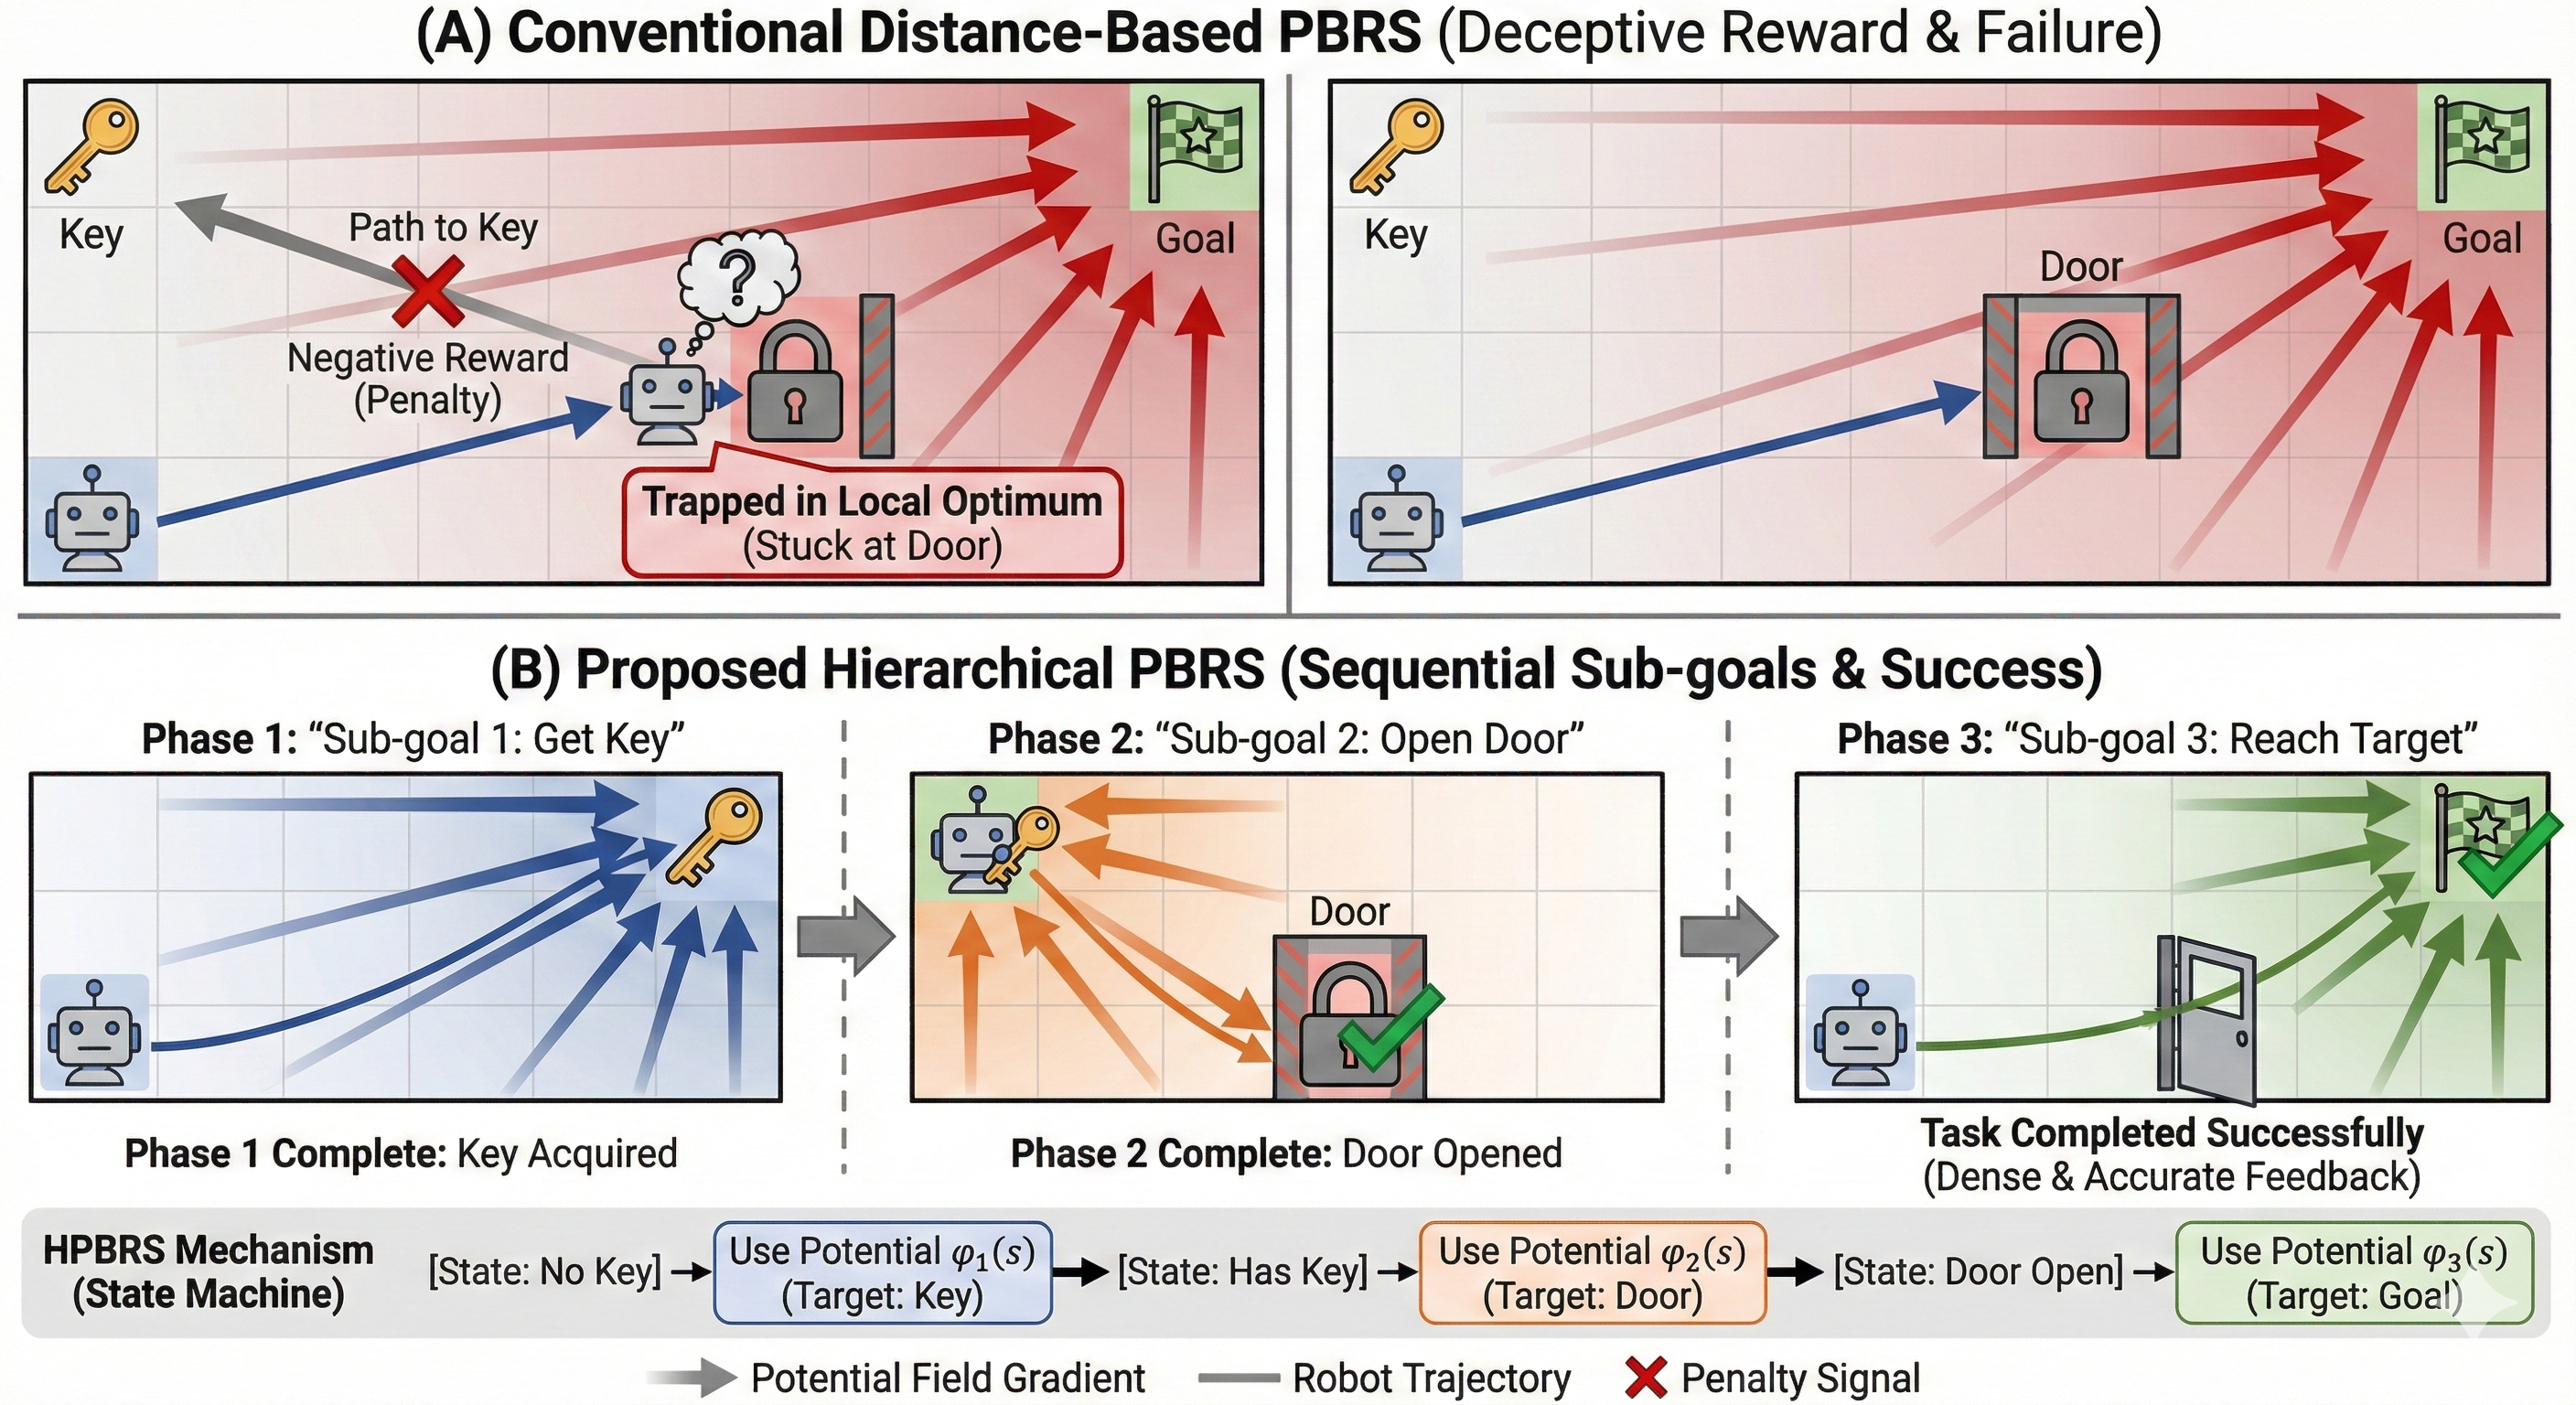
\includegraphics[width=0.7\linewidth]{figs/hpbrs_doorkey_comparison}
	\caption[Overcoming Deceptive Rewards in Long-Horizon Sequential Tasks via Hierarchical Potential-Based Reward Shaping (HPBRS).]{(A) Failure of Conventional Distance-Based PBRS. In the DoorKey task, a simple Euclidean distance potential field pulls the agent directly towards the final goal. This creates a deceptive reward signal (indicated by the red "X") that penalizes necessary deviations to fetch the key, causing the agent to become trapped in a local optimum near the locked door. (B) Success of Proposed HPBRS. Our method decomposes the task into sequential sub-goals (Get Key $\to$ Open Door  $\to$ Reach Target). By applying stage-specific potential functions, HPBRS provides accurate, dense feedback for each phase, guiding the agent successfully through the long-horizon dependency without altering the optimal policy.}
	\label{fig:hpbrsdoorkeycomparison}
\end{figure}

本文的主要贡献如下:

\begin{enumerate}
	
	\item 提出了一种通用的分层势能塑形框架,有效解决了顺序决策任务中简单距离塑形导致的局部最优问题。
	\item 在 MiniGrid-DoorKey 环境中进行了系统性验证。实验表明,在极具挑战性的 $8 \times 8$ 环境中,基线算法(PPO)和简单塑形方法完全失败(成功率为 0\%),而我们的方法实现了 100\% 的成功率。
	\item 与最先进的好奇心探索算法 RND (Random Network Distillation) 进行了对比,证明了在结构化任务中,精准的领域引导显著优于盲目的通用探索。
\end{enumerate}







\section{相关工作 (Related Work)}
\label{sec:related}
% 1. Sparse Reward RL (Curiosity, RND...)
% 2. Reward Shaping (Ng et al. 1999, PBRS)
% 3. Hierarchical RL (Options, Sub-goals)

\subsection{稀疏奖励与内在动机}

在稀疏奖励任务中,传统的 $\epsilon$-greedy 探索策略往往效率低下。为了解决这一问题,研究者提出了多种内在动机(Intrinsic Motivation)方法,如基于计数的方法和基于预测误差的方法。其中,随机网络蒸馏 (RND) 是一种代表性算法,它通过最大化预测误差来鼓励智能体访问新奇状态。然而,这类“好奇心”驱动的方法通常是语法性 (Syntactic) 而非语义性 (Semantic) 的。在状态空间巨大的环境中(如本文的 $8 \times 8$ 网格),智能体可能会被无关的新奇状态(如墙角的空地)吸引,而忽略了任务关键的瓶颈(如钥匙)。与此不同,本文的方法利用任务的逻辑结构直接引导智能体关注关键子目标。

%Prompt:
%Style: A professional, high-contrast technical diagram in the style of a top-tier AI conference paper (NeurIPS, ICML). Clean vector graphics, academic color palette (blues, oranges, grays, light reds), sans-serif typography. The figure is divided into two panels side-by-side, labeled (A) and (B).
%Overall Environment Setup (Both Panels): An $8 \times 8$ grid-world environment representing a sparse reward task. It contains:
%Empty grey grid cells.
%Black solid blocks representing "Walls".
%A small blue circle icon representing the Robot Agent (Start).
%A yellow icon representing a "Key" (the critical bottleneck) located in a narrow passage.
%A green flag icon representing the final "Goal" (behind a locked door area that requires the key).
%Panel (A) Title: (A) Curiosity-Driven Exploration (e.g., RND): Syntactic Novelty Distraction
%Panel (A) Visuals:
%Mechanism (Diffuse Heatmap): Overlaid on the grid is a diffuse, clouded heatmap representing intrinsic reward. Bright red/orange areas (high novelty) are spread out in irrelevant empty corners and along walls far from the key, indicating "syntactic" novelty. The area around the "Key" has some warmth but is not the sole focus.
%Agent Trajectory (Inefficient): A tangled, meandering blue dashed line shows the robot's path. The robot spends much time exploring the bright red, irrelevant corners, getting distracted. It passes near the key but misses it, drawn away by another "novel" empty corner.
%Labels: An arrow points to a red corner with text "Irrelevant 'New' State (High Intrinsic Reward)". Another label near the robot reads "Syntactic Exploration (Distracted)".
%Panel (B) Title: (B) Proposed Approach: Task Structure Guidance (Semantic Focus)
%Panel (B) Visuals:
%Mechanism (Focused Gradient): Instead of a heatmap, there is a clean, sharp field of thick blue arrows representing the guidance signal. These arrows point strongly and directly only towards the "Key" icon, ignoring the irrelevant corners completely. This indicates "semantic" importance.
%Agent Trajectory (Efficient): A direct, solid blue line shows the robot moving straight from the start position to the "Key", following the arrows efficiently.
%Labels: An arrow points to the focused arrow field near the key with text "Critical Sub-goal Focus (Semantic Guidance)". Another label near the robot reads "Efficient Bottleneck Reaching".
%Legend (Bottom Center): A small legend box. "Blue Dashed Line: Exploration Path", "Blue Solid Line: Guided Path", "Red/Orange Heatmap: Syntactic Novelty (RND)", "Blue Arrows: Semantic Structure Guidance (Ours)".

\begin{figure}[H]
	\centering
	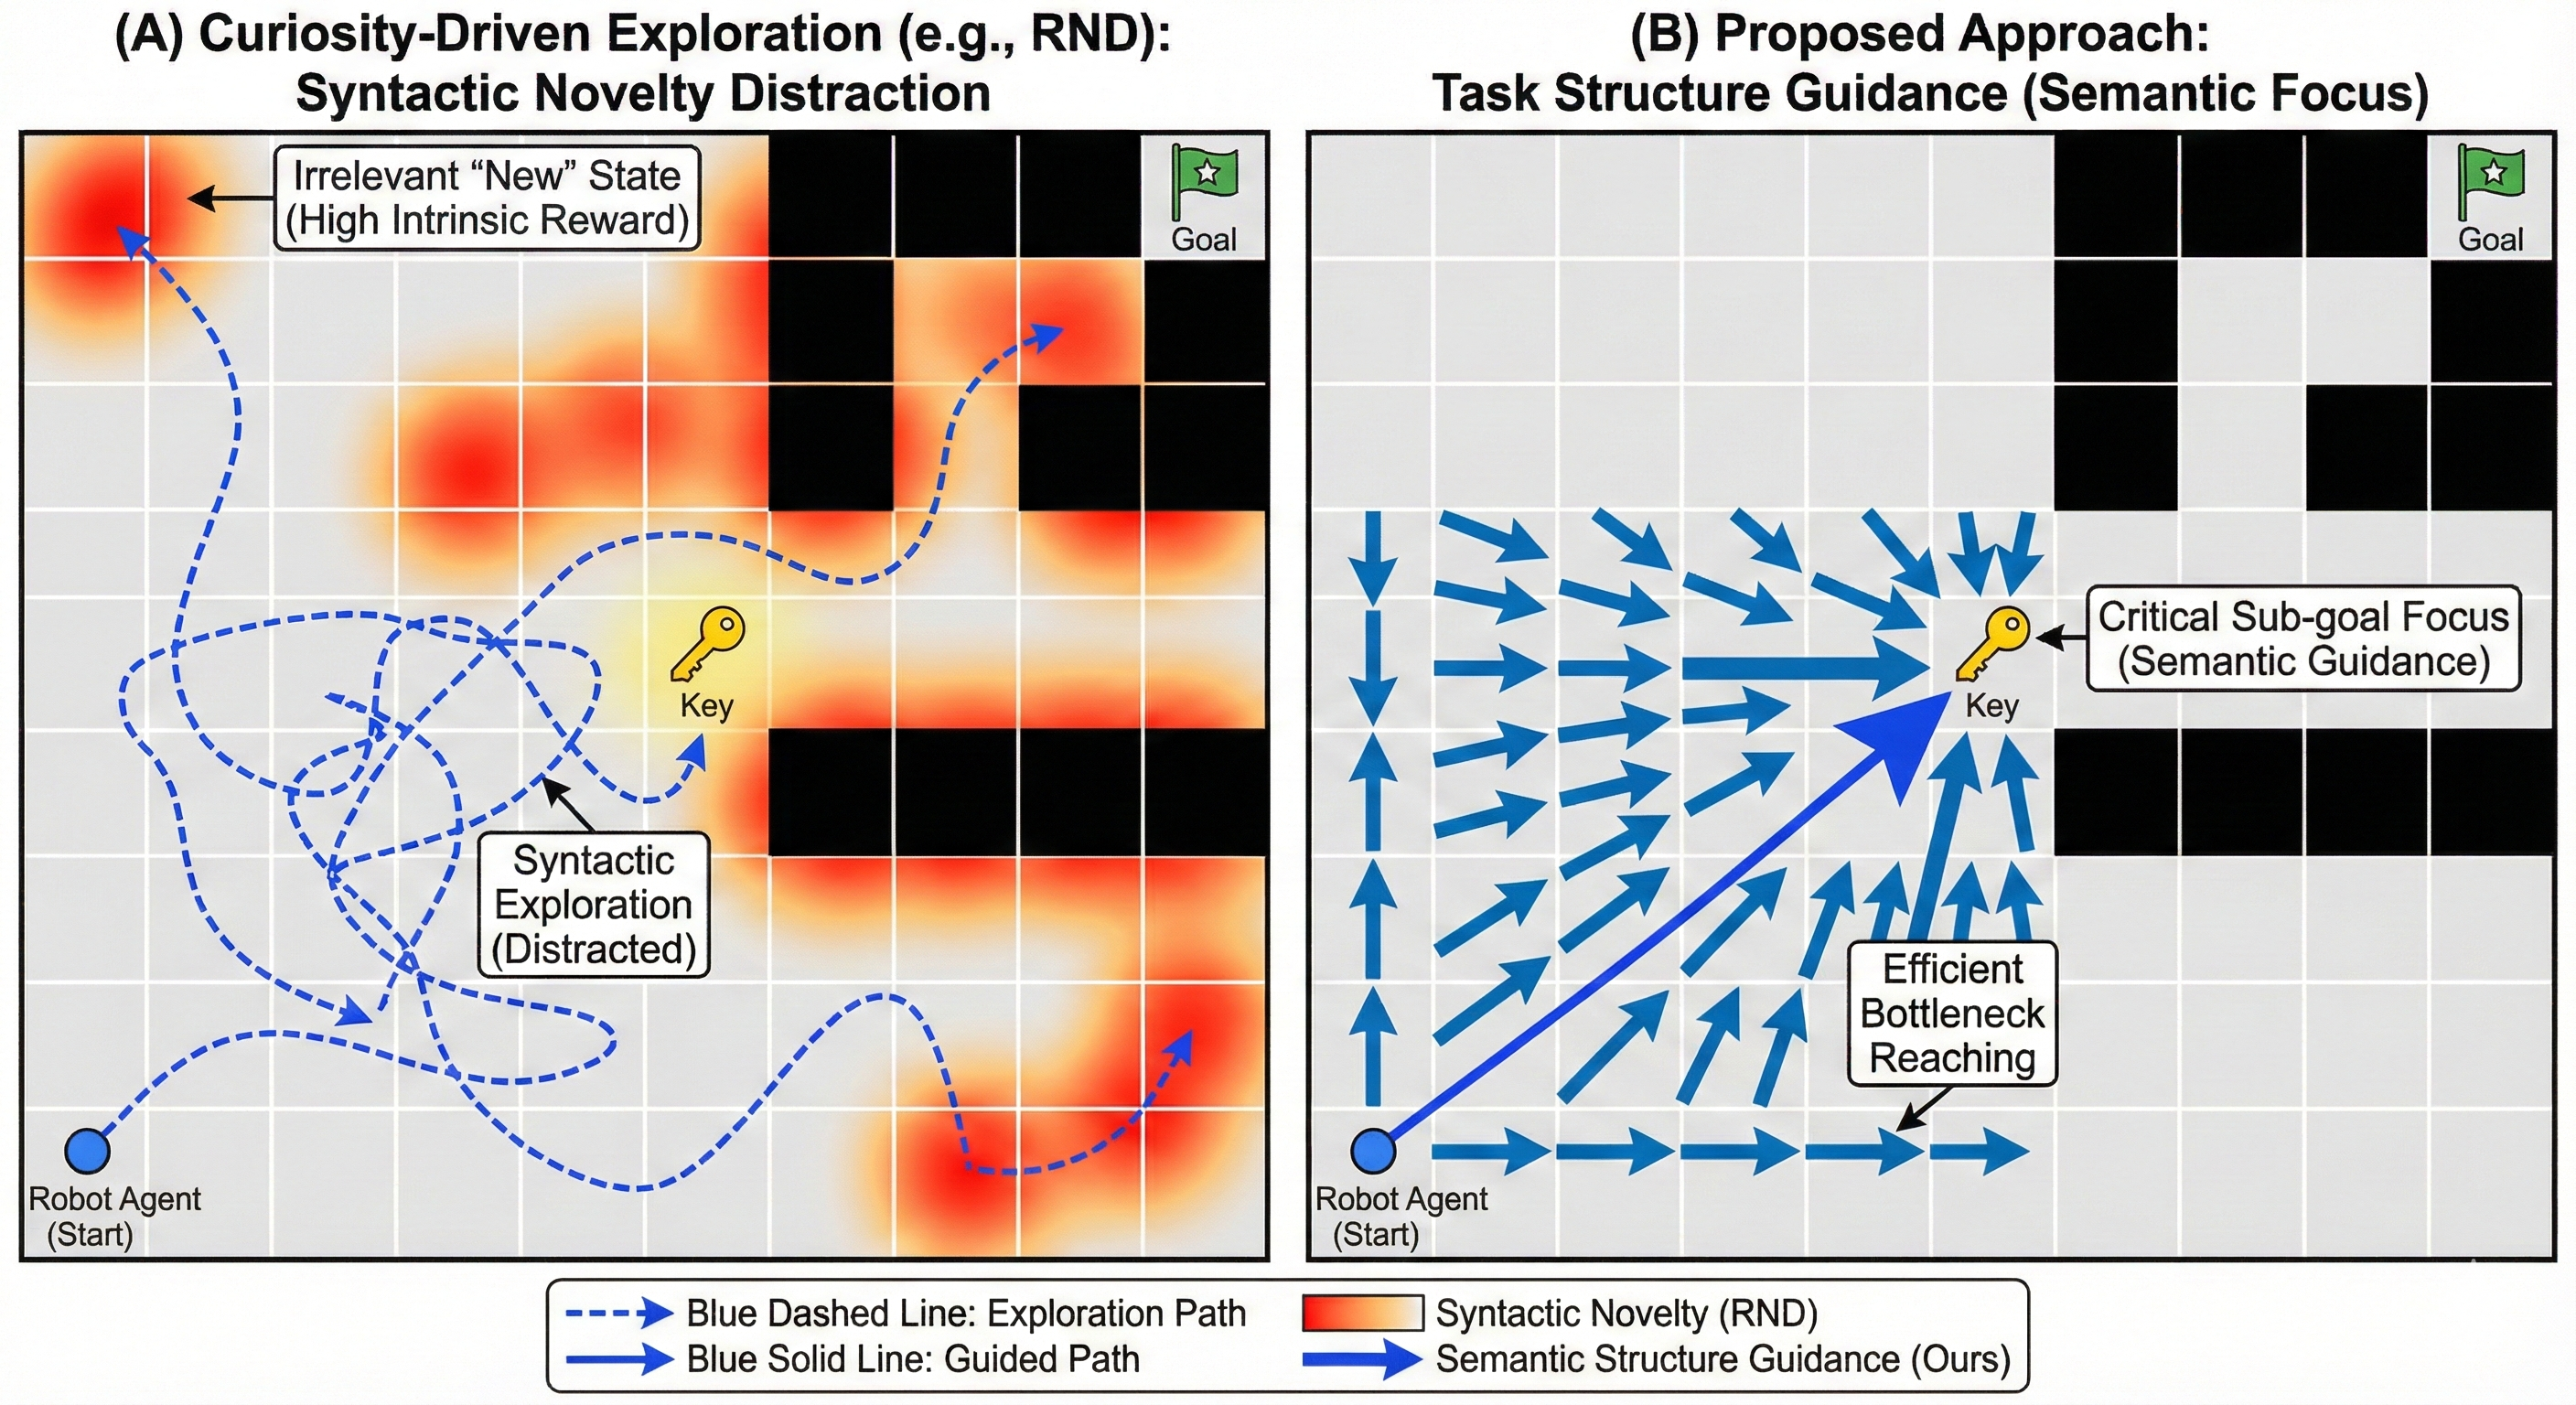
\includegraphics[width=0.7\linewidth]{figs/syntactic_vs_semantic_guidance}
	\caption[Contrast between Syntactic Novelty-Driven Exploration (RND) and Semantic Task Structure Guidance in a Large ($8 \times 8$) Sparse Reward Grid.]{(A) Distraction by Syntactic Novelty (RND). Conventional intrinsic motivation methods like RND encourage visiting novel states to maximize prediction error (shown by the diffuse heatmap). In a large state space, the agent is easily distracted by irrelevant novel areas (e.g., empty corners) and fails to efficiently reach the critical task bottleneck (the Key). (B) Focused Semantic Guidance (Ours). Our method leverages the logical structure of the task to provide focused guidance toward critical sub-goals. The agent ignores irrelevant states and moves directly to the bottleneck, demonstrating semantic understanding of the task.}
	\label{fig:syntacticvssemanticguidance}
\end{figure}

\subsection{奖励塑形与势能函数}

奖励塑形通过向原始奖励添加辅助信号来加速学习。为了避免改变最优策略,Ng 等人提出了基于势能的奖励塑形 (PBRS),证明了只要塑形奖励以势能差的形式存在,最优策略保持不变。虽然 PBRS 提供了理论保证,但势能函数的设计仍然是一个难题。现有的工作大多依赖简单的启发式规则(如欧几里得距离)。正如本文实验所示,在具有障碍物或顺序依赖的环境中,简单的距离势能会形成局部最优陷阱(Local Optima)。本文通过引入分层结构改进了势能函数的设计,消除了这种局部最优。

%Prompt:
%Style: A clean, professional schematic figure for a top-tier AI conference paper (NeurIPS/ICML style). High-contrast vector graphics, academic blue/orange/grey color palette, sans-serif typography. The figure is divided into two panels, (A) and (B), side-by-side with a shared legend.
%Environment Setup (Both Panels): A 2D plane with a Start position (small blue circle, bottom left), a Goal position (green flag, top right), and a large, grey, U-shaped obstacle barrier located between them. The open end of the "U" faces right.
%Panel (A) Title: (A) Standard Euclidean Potential (Local Optima Trap)
%Panel (A) Visuals:
%Potential Field Gradient: A field of thick red arrows covers the entire environment. All arrows point straight towards the final Goal flag, ignoring the obstacle geometry. This represents the gradient of simple distance-based potential $\nabla\Phi_{dist}(s)$.
%Agent Behavior: A robot icon is shown stuck deep inside the "U" shape barrier. A red circular highlight around it is labeled "Trapped in Local Optimum". A small trajectory line shows it moved straight in and stopped.
%Mechanism Note: A small text box indicates: "Moving around obstacle increases distance = Negative shaped reward."
%Panel (B) Title: (B) Proposed Hierarchical Potential (Trap Elimination)
%Panel (B) Visuals:
%Sub-goal: An intermediate "Sub-goal" marker (small yellow diamond) is placed at the open corner of the U-shape barrier, bridging the path to the goal.
%Hierarchical Potential Gradient: The field of arrows is now blue.
%In the left half (before the obstacle), blue arrows point strongly towards the Sub-goal.
%In the right half (after passing the sub-goal), blue arrows point towards the final Goal.
%Agent Behavior: A smooth blue solid trajectory line shows the robot moving from Start, curving around the U-shape barrier via the Sub-goal, and successfully reaching the Goal flag.
%Mechanism Note: A small text box indicates: "Potential guides to sequence of sub-goals = Continuous positive guidance."
%Legend (Bottom Center):
%[Red Arrow] $\nabla\Phi$ (Simple Distance), [Blue Arrow] $\nabla\Phi_{H}$ (Hierarchical), [Grey Block] Obstacle.

\begin{figure}[H]
	\centering
	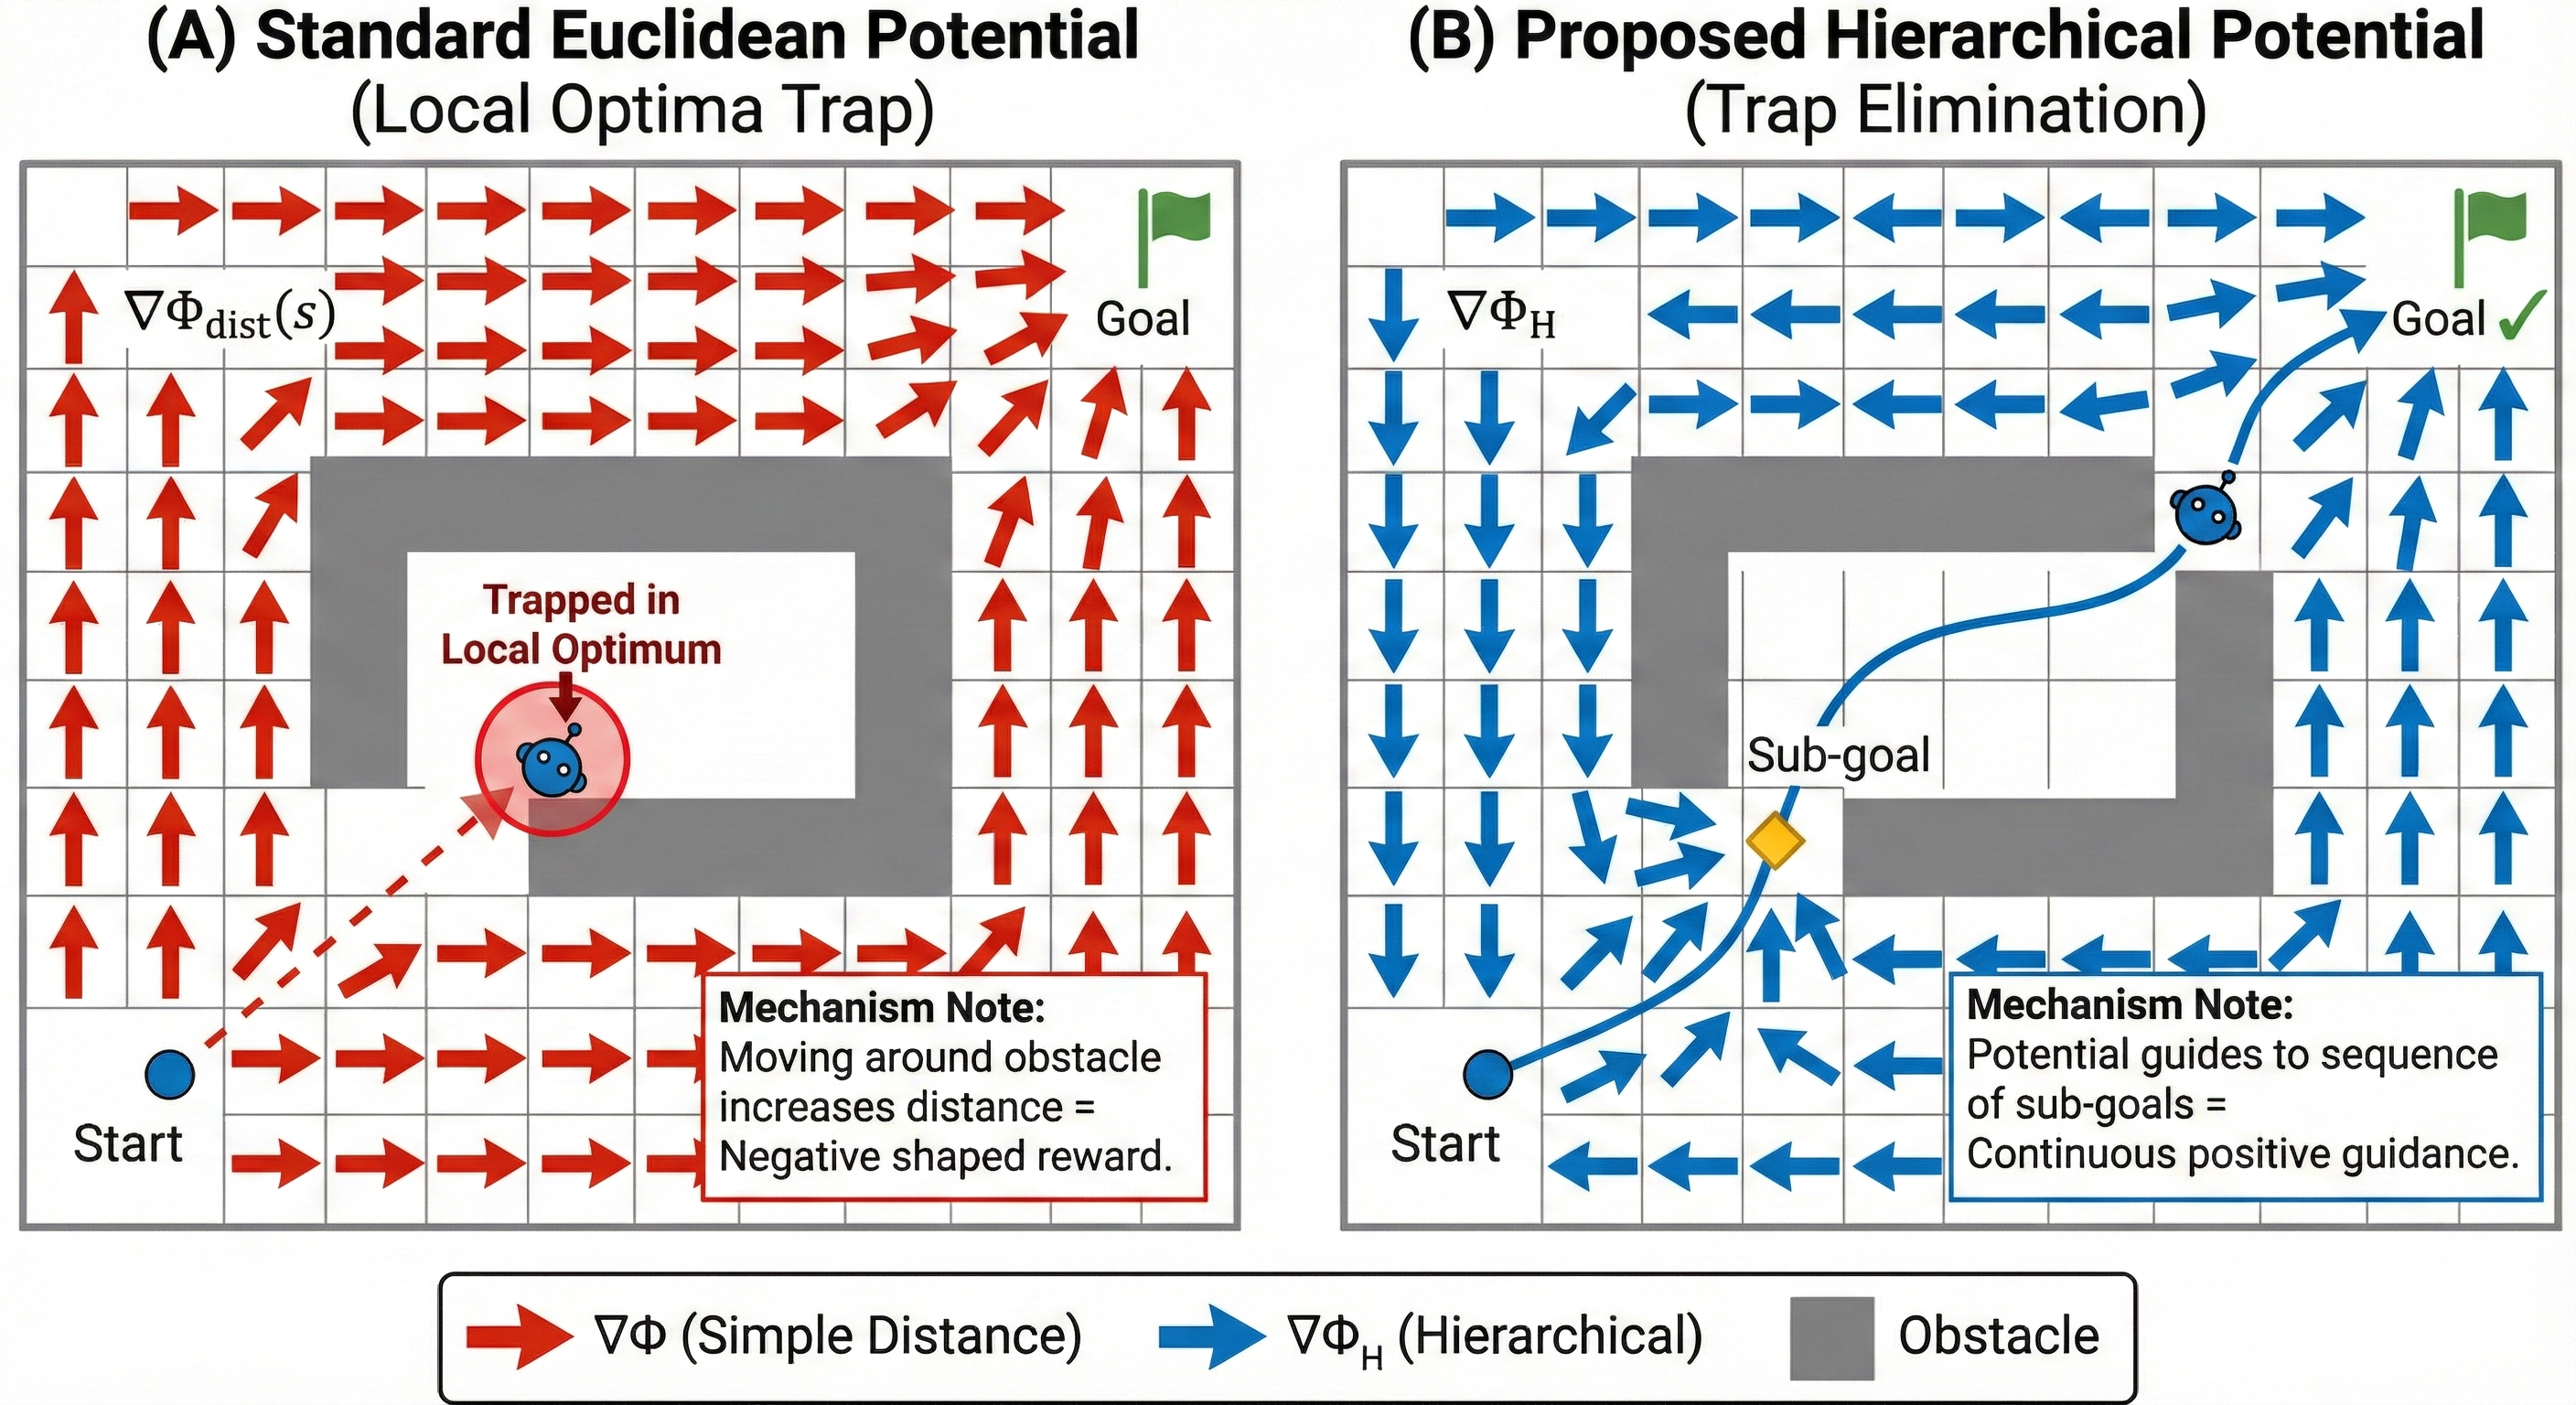
\includegraphics[width=0.7\linewidth]{figs/pbrs_local_optima_trap}
	\caption[Impact of Potential Function Design on Local Optima in Obstacle Environments.]{(A) Local Optima Trap with Euclidean Potential. Standard PBRS using simple Euclidean distance creates a gradient field (red arrows) that pulls the agent directly into the U-shaped obstacle. Escaping the obstacle requires moving away from the goal (increasing distance), which generates negative shaping rewards, trapping the agent. (B) Trap Elimination via Hierarchical Potential. Our proposed method directs the potential field (blue arrows) towards an intermediate sub-goal at the obstacle's opening. This preserves a continuous positive gradient, allowing the agent to bypass the obstacle and reach the target smoothly.}
	\label{fig:pbrslocaloptimatrap}
\end{figure}

\subsection{分层强化学习 (HRL)}

解决长程任务的另一种思路是分层强化学习(HRL),例如 Options 框架或 Feudal Networks。这些方法通常需要同时训练上层策略(High-level Policy)和下层策略(Low-level Policy),导致训练不稳定且样本效率较低。相比之下,我们的方法不需要额外的策略网络,而是通过分层设计的奖励函数将任务知识直接注入到单一策略的学习中,具有更高的实现效率和稳定性。

\section{方法论 (METHODOLOGY)}
\label{sec:method}

本节首先将问题形式化为马尔可夫决策过程,并回顾基于势能的奖励塑形(PBRS)的基础理论。随后,详细阐述我们提出的分层势能奖励塑形(HPBRS)方法,解释其如何通过整合领域知识来克服长程任务中的局部最优问题。

\subsection{Preliminaries (预备知识)}

\subsubsection{马尔可夫决策过程 (MDP)}
我们将智能体的顺序决策问题建模为马尔可夫决策过程 (MDP),由五元组 $\mathcal{M} = \langle \mathcal{S}, \mathcal{A}, \mathcal{P}, \mathcal{R}, \gamma \rangle$ 定义。其中,$\mathcal{S}$ 表示状态空间,$\mathcal{A}$ 表示动作空间,$\mathcal{P}: \mathcal{S} \times \mathcal{A} \times \mathcal{S} \to [0, 1]$ 是状态转移概率函数,$\mathcal{R}: \mathcal{S} \times \mathcal{A} \to \mathbb{R}$ 是环境反馈的奖励函数,$\gamma \in [0, 1)$ 是折扣因子。智能体的目标是学习一个最优策略 $\pi^*$,以最大化期望累积折扣回报:$J(\pi) = \mathbb{E}_{\pi}[\sum_{t=0}^{\infty} \gamma^t r_t]$。

\subsubsection{基于势能的奖励塑形 (PBRS)}
在稀疏奖励环境中,由于非零奖励极为罕见,标准强化学习算法往往收敛缓慢。奖励塑形通过在原始奖励 $\mathcal{R}$ 之上引入额外的辅助奖励 $F$ 来加速学习。为了确保塑形后的奖励不会改变原问题的最优策略(即策略不变性,Policy Invariance),Ng 等人提出了基于势能的奖励塑形(PBRS)。

PBRS 将辅助奖励定义为势能函数 $\Phi: \mathcal{S} \to \mathbb{R}$ 在连续状态下的差分形式:
\begin{equation}
	F(s, s') = \gamma \Phi(s') - \Phi(s)
\end{equation}
修正后的总奖励函数为 $R'(s, a, s') = R(s, a, s') + F(s, s')$。理论证明,在 $R'$ 下的最优策略与原奖励函数 $R$ 下的最优策略一致,这为我们设计复杂的势能函数提供了理论保障。


\subsection{简单塑形的局限性 (The Limitation of Simple Shaping)}
\label{subsec:limitation}

在导航任务中,一种常见的启发式方法是基于当前状态到最终目标的欧几里得距离或曼哈顿距离来定义势能 $\Phi_{simple}(s) = -dist(s, s_{goal})$。虽然这种方法在开阔空间中有效,但在具有顺序依赖的环境(如 DoorKey 任务)中会失效。

考虑这样一个场景:智能体必须背离最终目标移动去拾取钥匙。在这种情况下,$dist(s', s_{goal}) > dist(s, s_{goal})$,导致塑形奖励 $F(s, s') < 0$。这种惩罚在锁住的门附近制造了一个欺骗性的局部最优(Local Optima),阻碍智能体探索必要的子目标(钥匙)。

\begin{figure}[H]
    \centering
    \includegraphics[width=0.8\linewidth]{../verification_simple_shaping}
    \caption{\textbf{简单势能函数 $\Phi_S(s)$ 的验证。} 黄色实线(代码计算值)与灰色虚线(理论归一化距离)完全重合。关键在于,当智能体拿到钥匙时("Has Key" 脉冲处),势能值没有任何跳变,证实了简单距离塑形无法对子目标完成提供正向反馈。}
    \label{fig:verificationsimpleshaping}
\end{figure}

为了验证这一局限性,我们在随机游走过程中记录了简单势能函数的数值变化。如图 \ref{fig:verificationsimpleshaping} 所示,两个关键观察证实了其缺陷:

\begin{enumerate}
    \item \textbf{几何一致性 (Geometric Consistency):} 计算出的势能(黄色实线)与理论距离(灰色虚线)完美重合,表明该函数严格反映了与终点的几何关系,而忽略了环境的拓扑结构(如墙壁阻隔)。
    \item \textbf{对子目标的忽视 (Ignorance of Sub-goals):} 最关键的是,当智能体获取钥匙时(图中 "Has Key" 脉冲所示时刻),势能值没有表现出任何跳变或增长。这意味着基于简单距离的势能无法为完成子目标提供激励反馈,解释了为什么使用该方法的智能体难以逃离门前的局部最优。
\end{enumerate}

这一发现表明,必须引入包含领域知识的分层结构,才能在长程任务中提供有效的引导。

\subsection{Hierarchical Potential-Based Reward Shaping (分层势能奖励塑形)}

在具有顺序依赖的任务(如 DoorKey 环境)中,简单的基于“目标距离”的启发式势能往往会失效。例如,当智能体需要背离最终目标去拾取钥匙时,距离势能会产生负奖励,形成局部最优陷阱。为了解决这一冲突,我们提出了分层势能奖励塑形(HPBRS)。

\subsubsection{任务分解与阶段定义}
我们将长程任务分解为 $K$ 个顺序子目标序列 $\{g_0, g_1, \dots, g_{K-1}\}$,其中 $g_{K-1}$ 为最终目标。针对 DoorKey 任务,我们定义以下三个阶段($K=3$):

%Prompt:
%Style: Top-tier AI conference schematic (NeurIPS style). Flat 2D vector graphics, clean layout, horizontal flow.
%Layout: Three square panels arranged horizontally, connected by arrows labeled "Transition".
%Panel 1 (Left) - Stage 0:
%Visual: A grid showing the Robot (blue circle) and the Key (yellow icon). The Door is closed (red bar).
%Highlight: A dashed arrow points from Robot to Key.
%Label: Bold text "Stage 0: Get Key". Subtext: "Sub-goal $g_0$ = Key Pos".
%Panel 2 (Middle) - Stage 1:
%Visual: The Robot now has a small key icon attached to it. The Key is gone from the map. The Door is still closed.
%Highlight: A dashed arrow points from Robot to Door.
%Label: Bold text "Stage 1: Open Door". Subtext: "Sub-goal $g_1$ = Door Pos". Base potential label: "$C_1 > C_0$".
%Panel 3 (Right) - Stage 2:
%Visual: The Door is now Open (green translucent bar). The Robot is at the door threshold. The Goal (green flag) is visible.
%Highlight: A dashed arrow points from Robot to Goal.
%Label: Bold text "Stage 2: Reach Goal". Subtext: "Sub-goal $g_2$ = Goal Pos". Base potential label: "$C_2 > C_1$".
%Color Palette: Professional Slate Blue, Teal, and Soft Orange.

\begin{figure}[H]
	\centering
	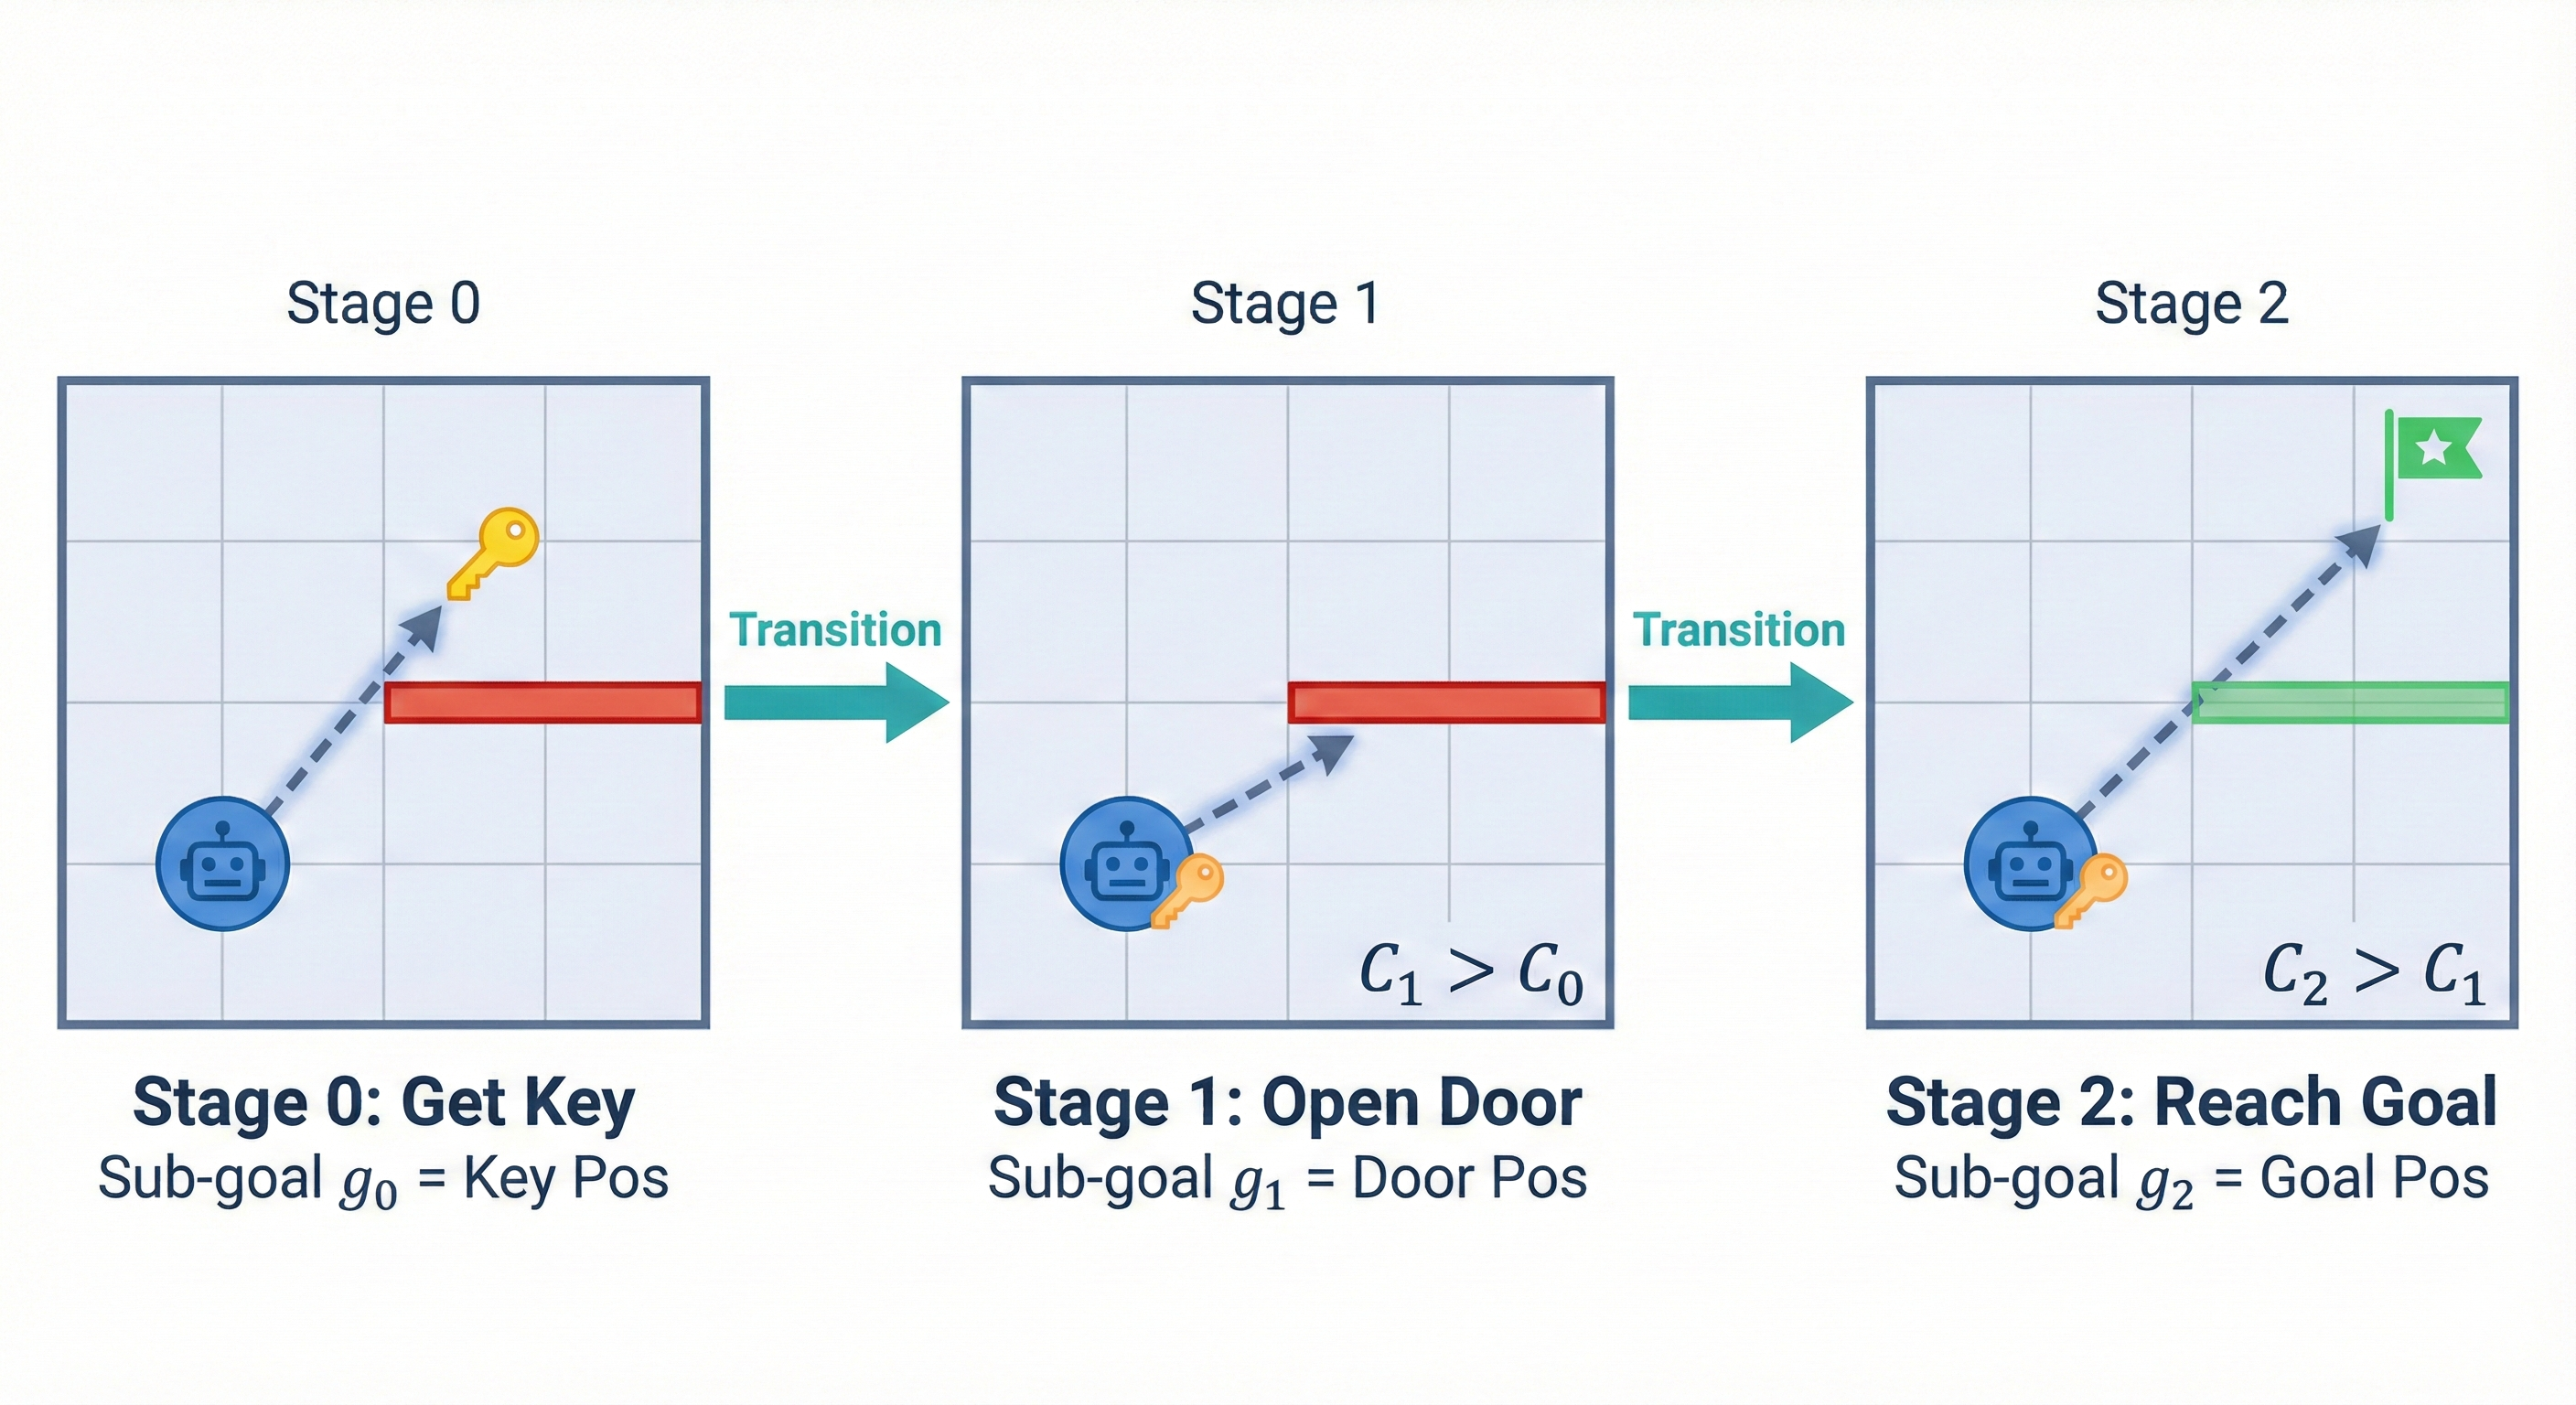
\includegraphics[width=0.7\linewidth]{figs/hpbrs_stage_decomposition}
	\caption[Sequential Task Decomposition in DoorKey Environment.]{The task is divided into three stages: retrieving the key ($k=0$), opening the door ($k=1$), and reaching the goal ($k=2$).}
	\label{fig:hpbrsstagedecomposition}
\end{figure}



\begin{itemize}
	\item \textbf{Stage 0 (获取钥匙):} 智能体尚未持有钥匙。此时的子目标 $g_0$ 为钥匙的位置。
	\item \textbf{Stage 1 (开启门):} 智能体持有钥匙,但门处于关闭状态。此时的子目标 $g_1$ 为门的位置。
	\item \textbf{Stage 2 (到达终点):} 门已开启。此时的子目标 $g_2$ 为最终终点的位置。
\end{itemize}

\subsubsection{分层势能函数构建}
基于上述阶段,我们设计了一个分段式的分层势能函数 $\Phi_{H}(s)$。该函数不仅引导智能体向当前阶段的子目标移动,还在阶段切换时提供显著的奖励跳跃。数学定义如下:

\begin{equation}
	\Phi_{H}(s) = C_k + \omega \cdot \left( 1 - \frac{dist(s, g_k)}{D_{max}} \right)
\end{equation}

其中:
\begin{itemize}
	\item $k \in \{0, 1, 2\}$ 表示智能体在状态 $s$ 下所处的阶段索引。
	\item $g_k$ 是当前阶段对应的目标位置坐标。
	\item $dist(\cdot, \cdot)$ 表示曼哈顿距离 (Manhattan Distance)。
	\item $D_{max} = Width + Height$ 是网格环境的最大可能距离,用于归一化。
	\item $\omega$ 是距离权重的缩放系数(实验中设为 1.0)。
	\item $C_k$ 是阶段基准势能 (Stage Base Potential),用于区分不同阶段的价值层级。为了保证阶段推进时的正向激励,必须满足 $C_0 < C_1 < C_2$。在实验中,我们将 $C_k$ 简单设定为阶段索引值,即 $C_0=0, C_1=1, C_2=2$。
\end{itemize}

%Prompt:
%Style: A conceptual 3D surface plot schematic with white background. Clean, isometric view. High contrast.
%Content: A "Staircase" consisting of three separated, floating planes (surfaces) arranged stepwise from bottom-left to top-right.
%Plane 1 (Bottom) - Stage 0:
%Look: A semi-transparent blue grid surface. It is tilted slightly upwards.
%Details: The lowest point is "Start". The highest point on this plane is labeled "$g_0$ (Key)".
%Label: "Stage 0 Potential ($C_0=0$)" floating next to it.
%Plane 2 (Middle) - Stage 1:
%Look: An orange grid surface floating significantly higher than Plane 1.
%Details: A vertical dashed line connects $g_0$ on Plane 1 to the start of Plane 2. This plane slopes upwards to a point labeled "$g_1$ (Door)".
%Label: "Stage 1 Potential ($C_1=1$)" floating next to it.
%Plane 3 (Top) - Stage 2:
%Look: A green grid surface floating even higher.
%Details: A vertical dashed line connects $g_1$ on Plane 2 to the start of Plane 3. This plane slopes upwards to the final point labeled "$g_2$ (Goal)".
%Label: "Stage 2 Potential ($C_2=2$)".
%Annotations: Add curly braces or arrows indicating the vertical gaps as "Inter-stage Bonus ($C_{k+1} - C_k$)" and the slope on the planes as "Intra-stage Gradient".

\begin{figure}[H]
	\centering
	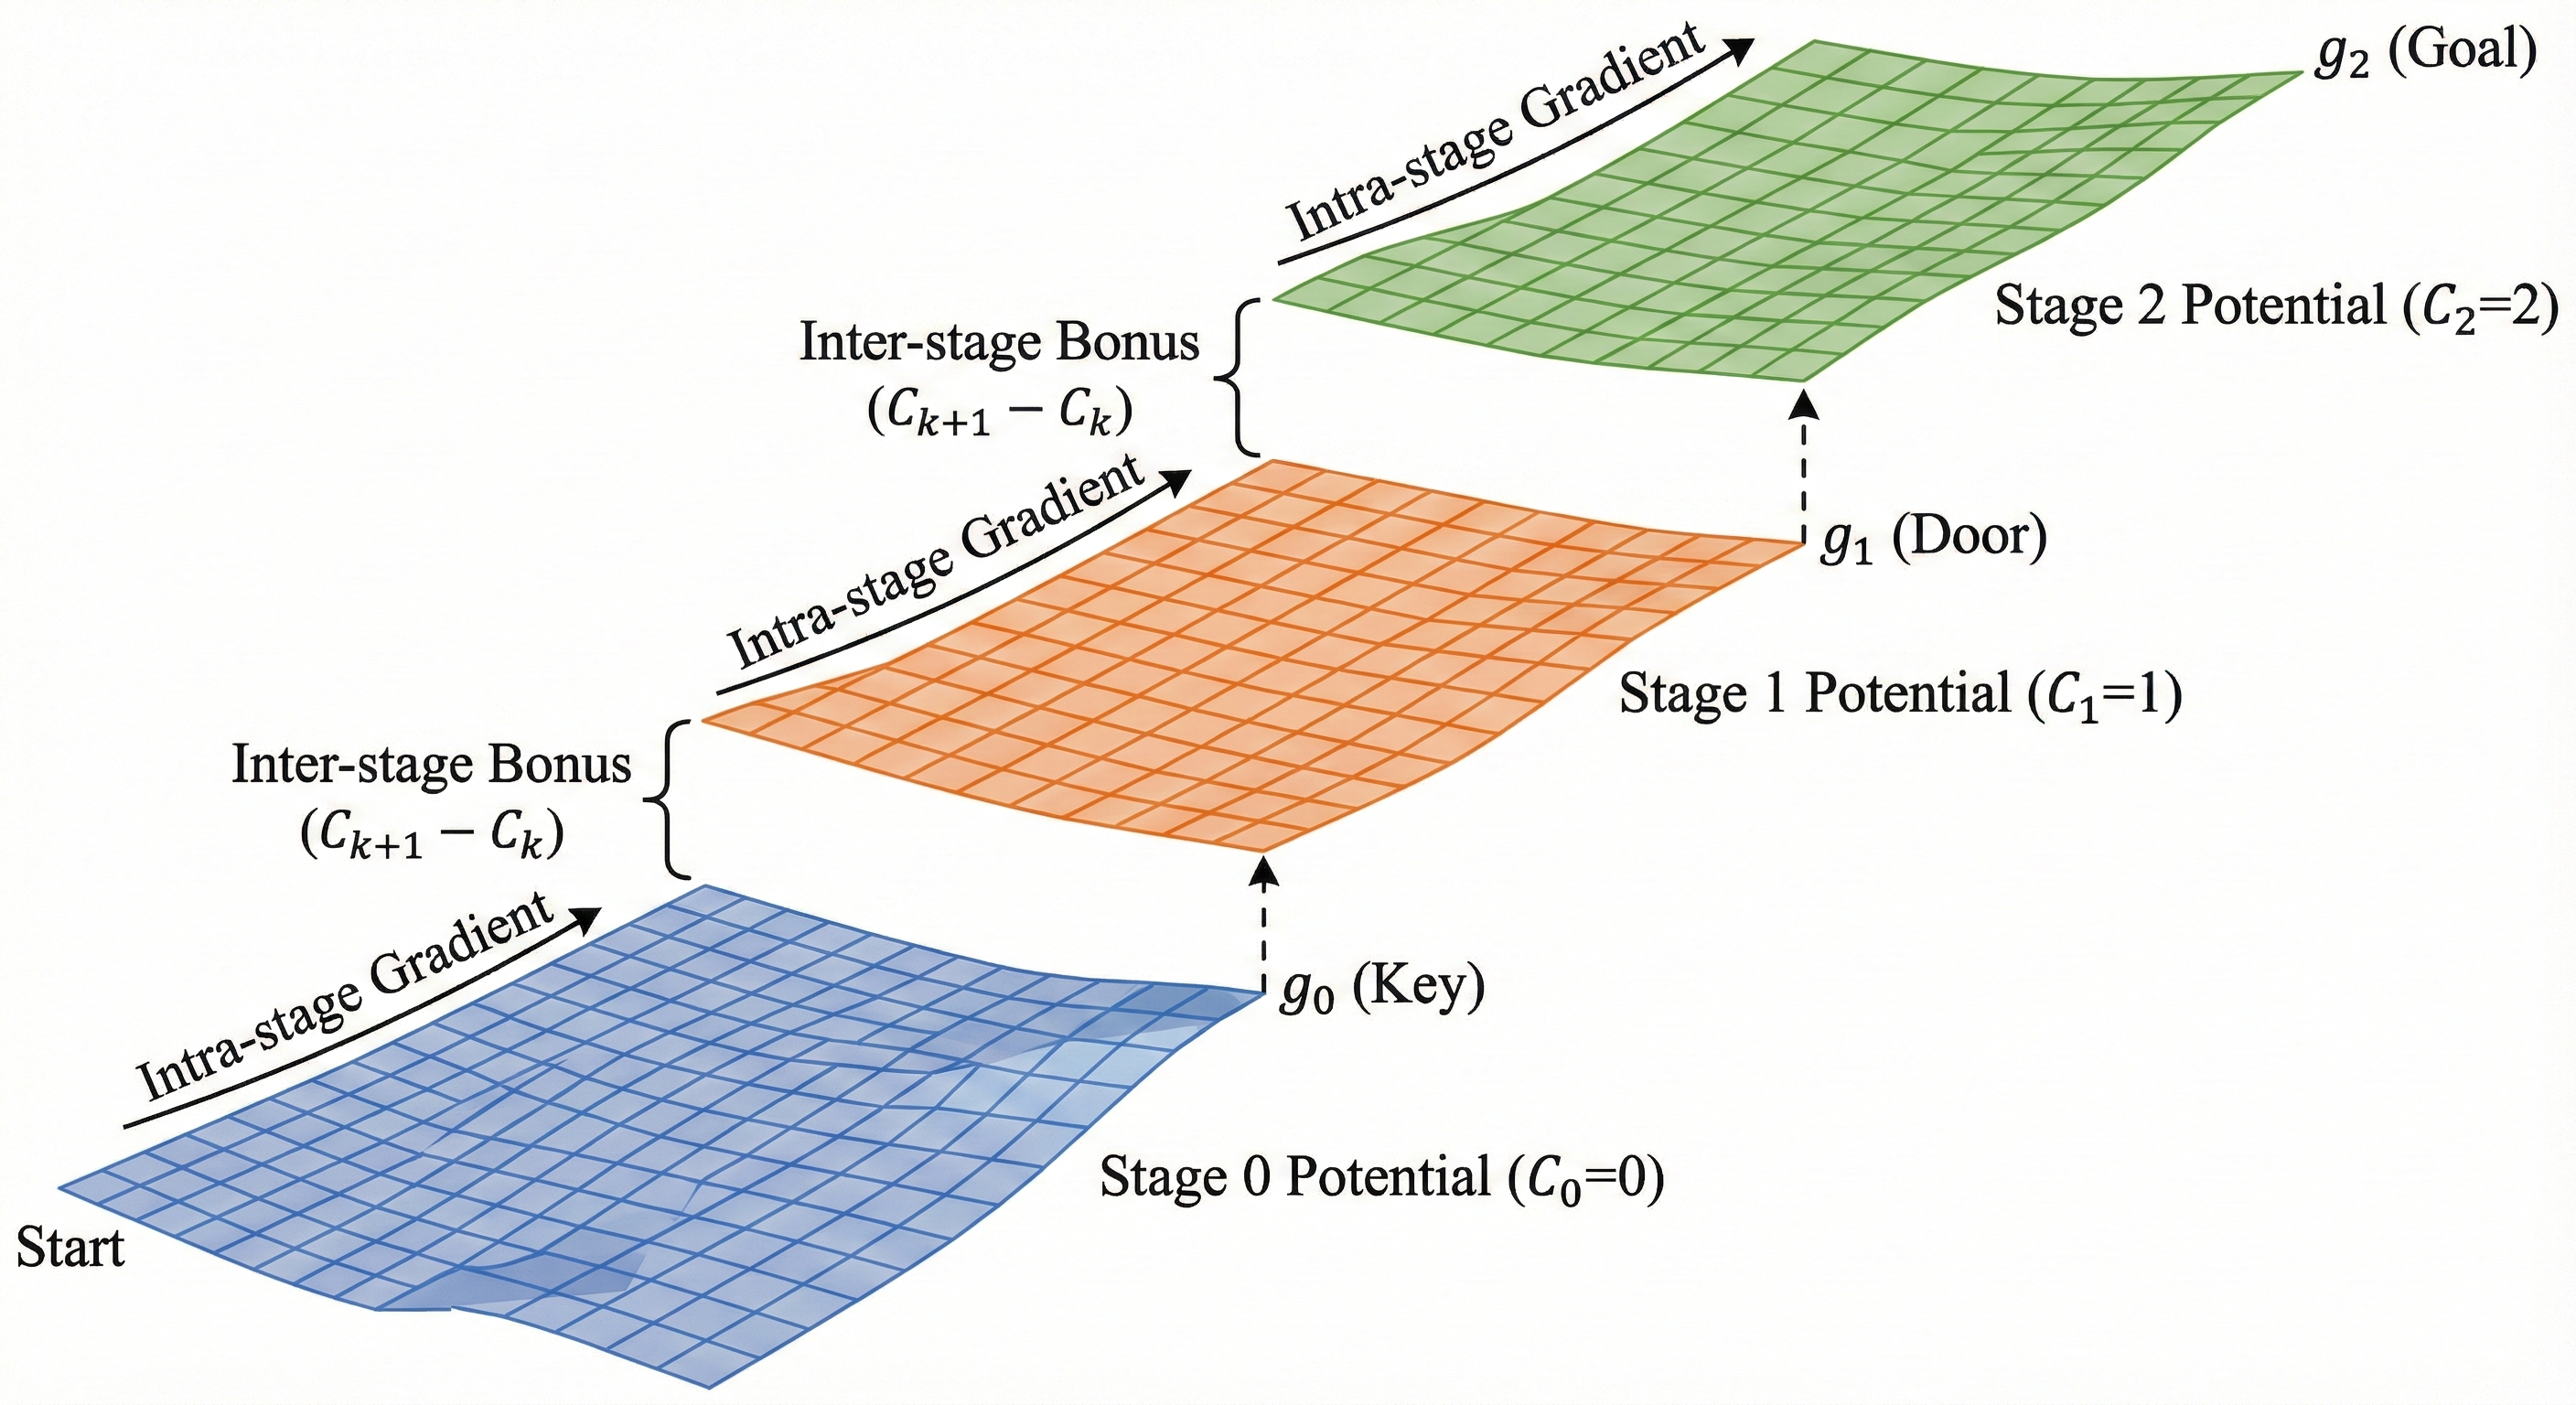
\includegraphics[width=0.7\linewidth]{figs/potential_function_landscape}
	\caption[The Staircase Structure of Hierarchical Potential Function $\Phi_{H}(s)$.]{Each stage operates on a higher potential plane ($C_0 < C_1 < C_2$). Intra-stage potential guides the agent to the sub-goal, while inter-stage transitions provide a vertical potential jump, preventing backward movement.}
	\label{fig:potentialfunctionlandscape}
\end{figure}


% \subsubsection{机制分析}
% $\Phi_{H}(s)$ 的设计通过两种机制促进学习:
% \begin{enumerate}
% 	\item \textbf{阶段内梯度引导 (Intra-stage Gradient):} 在同一阶段 $k$ 内,随着智能体靠近子目标 $g_k$,项 $-dist(s, g_k)$ 增大,产生的塑形奖励 $F > 0$,引导智能体沿最短路径移动。
% 	\item \textbf{阶段间跳跃奖励 (Inter-stage Bonus):} 当智能体完成子目标(例如捡起钥匙)并从阶段 $k$ 跃迁至 $k+1$ 时,基准势能从 $C_k$ 突变至 $C_{k+1}$。这将产生一个巨大的正向塑形奖励 $F \approx C_{k+1} - C_k$,强烈强化了完成子目标这一关键行为。
% \end{enumerate}

% %Prompt:Style: A technical data plot/chart typical of scientific papers. Minimalist, clear axis labels.Content: A line graph showing "Shaping Reward $F$" (Y-axis) over "Time Steps" (X-axis).The Curve:Segment 1 (Approaching Key): A jagged but generally positive line (representing the gradient guidance).Event 1 (Key Picked): A sharp, tall vertical Green Spike. Label this spike: "Inter-stage Bonus (Jump to $C_1$)".Segment 2 (Approaching Door): The line returns to a lower baseline but remains positive/stable as it moves to the door.Event 2 (Door Opened): Another sharp, tall vertical Green Spike (Higher than the first if possible, or same size). Label: "Inter-stage Bonus (Jump to $C_2$)".Segment 3 (To Goal): Positive line leading to the end.Annotations: Use a bracket over the low-level positive segments labeled "Intra-stage Gradient Guidance".Visual Aid: Small icons (Key, Door) placed on the X-axis at the moments where the spikes occur to correlate the event with the signal.

% \begin{figure}[H]
% 	\centering
% 	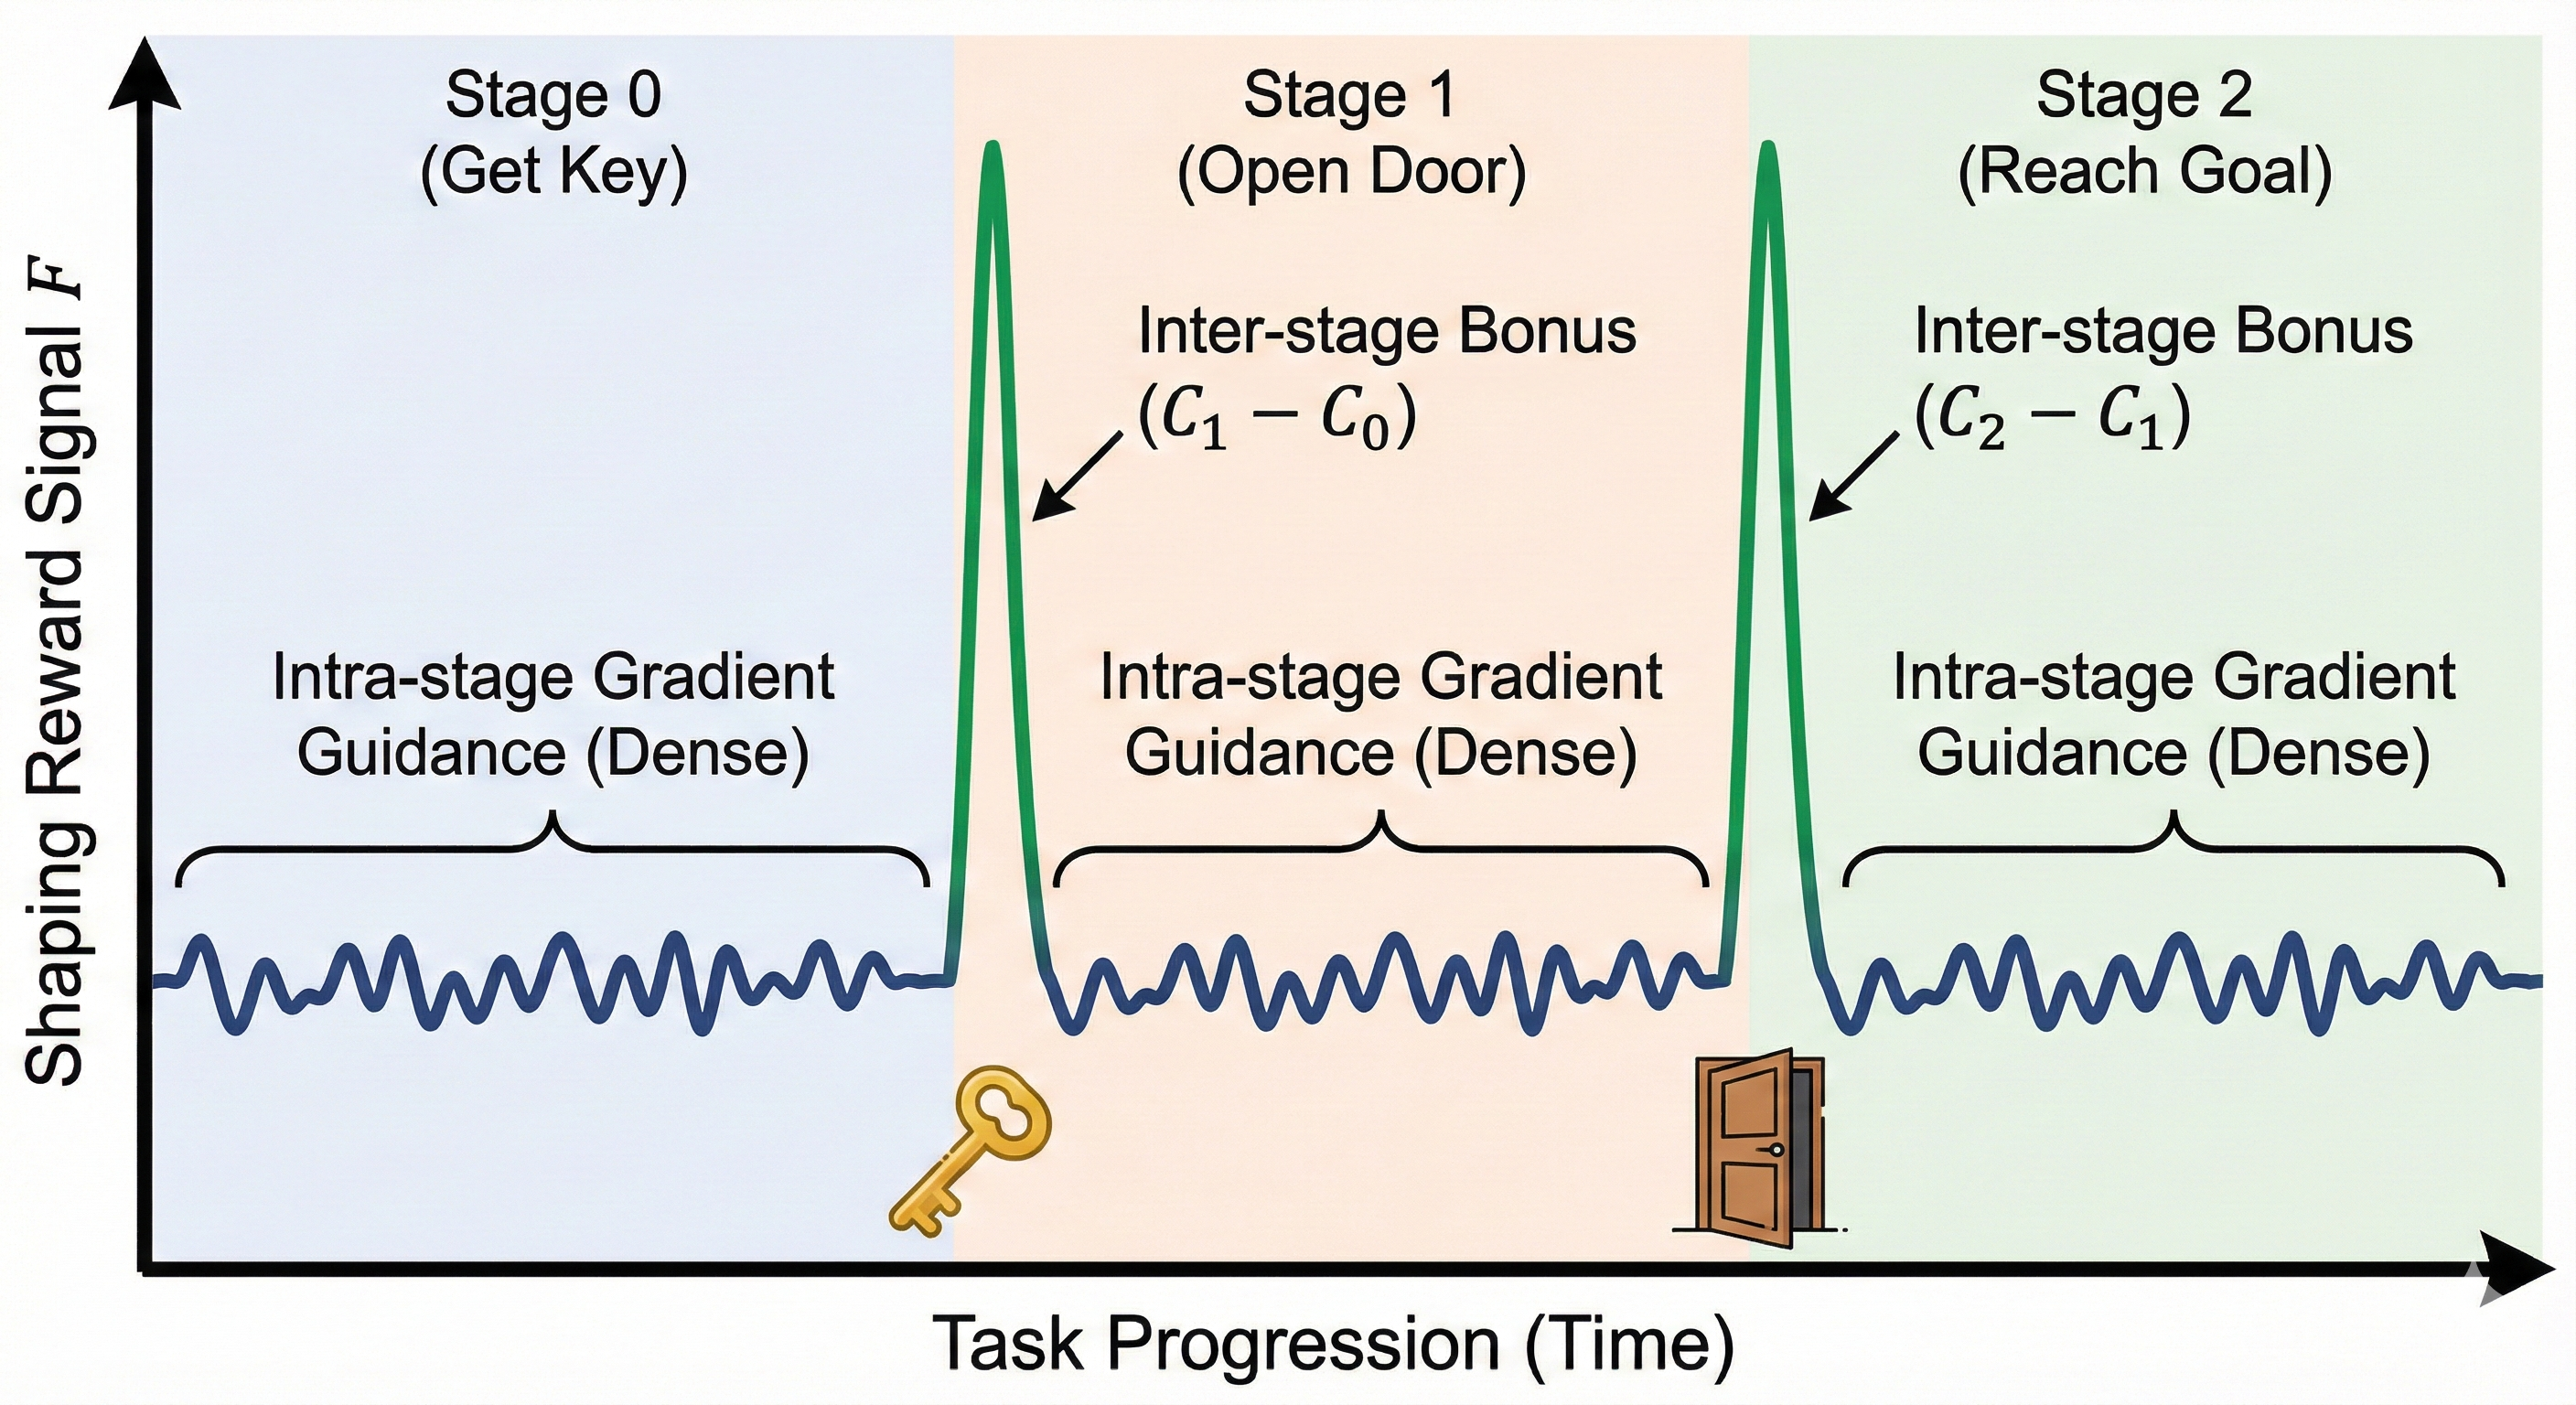
\includegraphics[width=0.7\linewidth]{figs/shaping_reward_mechanism_schematic}
% 	\caption[Conceptual Illustration of HPBRS Reward Dynamics.]{The mechanism provides continuous gradient guidance within stages (low amplitude) and delivers significant bonus spikes (high amplitude) upon completing sub-goals to reinforce stage transitions.}
% 	\label{fig:shapingrewardmechanismschematic}
% \end{figure}

% 通过这种分层设计,HPBRS 成功消除了简单距离塑形中的“回溯惩罚”,使得智能体能够顺畅地跨越稀疏奖励的鸿沟。

\subsubsection{机制分析}
$\Phi_{H}(s)$ 的设计通过两种机制促进学习:
\begin{enumerate}
    \item \textbf{阶段内梯度引导 (Intra-stage Gradient):} 在同一阶段 $k$ 内,随着智能体靠近子目标 $g_k$,项 $-dist(s, g_k)$ 增大,产生的塑形奖励 $F > 0$,引导智能体沿最短路径移动。
    \item \textbf{阶段间跳跃奖励 (Inter-stage Bonus):} 当智能体完成子目标(例如捡起钥匙)并从阶段 $k$ 跃迁至 $k+1$ 时,基准势能从 $C_k$ 突变至 $C_{k+1}$。这将产生一个巨大的正向塑形奖励 $F \approx C_{k+1} - C_k$,强烈强化了完成子目标这一关键行为。
\end{enumerate}

\begin{figure}[H]
    \centering
    \includegraphics[width=0.8\linewidth]{../verification_hierarchical_shaping}
    \caption{\textbf{分层势能函数 $\Phi_H(s)$ 与塑形奖励 $F$ 的动态特性验证。} 上图显示势能值 $\Phi(s)$ 在子目标达成(拿钥匙、开门)时出现精确的阶跃;下图显示对应的塑形奖励 $F$ 在这些时刻产生尖锐的正向脉冲,提供了关键的强化信号。}
    \label{fig:verificationhierarchicalshaping}
\end{figure}

图 \ref{fig:verificationhierarchicalshaping} 验证了分层势能的多阶段机制。正如预期,势能值 $\Phi(s)$(上图)在子目标达成时出现了精确的离散跳变:在获取钥匙时从 $\approx 1.0$ 跳至 $\approx 2.0$,在开启门时从 $\approx 2.0$ 跳至 $\approx 3.0$。在每个阶段内部,势能随着智能体靠近下一个目标而平滑增长。相应地,塑形奖励 $F$(下图)在这些状态转换时刻表现出尖锐的正向脉冲(Spikes),为智能体完成序列子任务提供了强有力的即时反馈,这与前文简单塑形中缺失反馈的现象(图 \ref{fig:verificationsimpleshaping})形成了鲜明对比。

\section{实验 (Experiments)}
\label{sec:exp}


为了评估 HPBRS 方法的有效性、鲁棒性及通用性,我们在 MiniGrid 导航环境中设计了一系列层层递进的实验。我们主要关注两个核心指标:平均回合奖励 (Average Episodic Reward) 和 任务成功率 (Task Success Rate)。

\subsection{实验设置}
% MiniGrid 环境介绍
% 算法设置 (PPO/DQN, CNN架构)

我们选择了 MiniGrid-Empty-8x8(无障碍导航)和 MiniGrid-DoorKey(顺序依赖导航)作为测试环境。基线算法采用 PPO(Proximal Policy Optimization),并使用卷积神经网络(CNN)处理图像输入。我们将以下三种设置进行对比:

\begin{enumerate}
\item Baseline: 仅使用环境原始稀疏奖励的 PPO。

\item Simple Shaping: 使用基于“当前位置到最终目标距离”的势能塑形。
	
\item Ours (HPBRS): 使用本文提出的分层势能塑形。
\end{enumerate}

\begin{table}[H]
\caption{不同方法在 DoorKey 环境下的性能量化对比。指标包括:最终任务成功率 (Success Rate @ 500k) 和 达到 90\% 成功率所需的步数 (Steps to 90\%)。}
\label{tab:performance_summary}
\centering
\begin{tabular}{l|cc|cc}
\hline
\textbf{Environment} & \multicolumn{2}{c|}{\textbf{DoorKey-5x5}} & \multicolumn{2}{c}{\textbf{DoorKey-8x8}} \\
\cline{2-5} 
\textbf{Method} & \textbf{Success \%} & \textbf{Steps to 90\%} & \textbf{Success \%} & \textbf{Steps to 90\%} \\
\hline
Baseline & 100\% & $\approx$ 100k & 0\% & N/A \\
Simple Shaping & 100\% & $\approx$ 120k & 0\% & N/A \\
RND & 100\% & $\approx$ 110k & 0\% & N/A \\
\textbf{Ours (HPBRS)} & \textbf{100\%} & \textbf{$\approx$ 35k} & \textbf{100\%} & \textbf{$\approx$ 150k} \\
\hline
\end{tabular}
\end{table}

\subsection{学习效率验证 (MiniGrid-Empty-8x8)}

% 实验 1: 基础有效性 (Empty-8x8)
\begin{figure}[H]
	\centering
	\includegraphics[width=0.8\linewidth]{../logs_paper_minigrid_empty_8x8_v0_fixed.png}
	\caption{\textbf{Learning Efficiency on MiniGrid-Empty-8x8.} Our method accelerates convergence while maintaining policy invariance.}
	\label{fig:empty}
\end{figure}

首先,我们在简单的无障碍环境中验证方法的基础有效性。如图 \ref{fig:empty} 所示,HPBRS(红线)的收敛速度明显快于基线算法。更重要的是,两种方法最终收敛到了相同的最高分数,这验证了 PBRS 的策略不变性——即我们的塑形方法加速了学习,但没有引入会导致次优策略的偏差。

\subsection{机制解析与消融实验 (DoorKey-5x5)}

% 实验 2: 消融实验 (DoorKey-5x5)
\begin{figure}[H]
	\centering
	\includegraphics[width=0.8\linewidth]{../ablation_result_optimized.png}
	\caption{\textbf{Ablation Study on DoorKey-5x5.} Comparison showing our method outperforms simple shaping, which suffers from local optima (dip in performance).}
	\label{fig:ablation}
\end{figure}

在 $5 \times 5$ 的 DoorKey 环境中,我们深入分析了简单塑形的缺陷(如图 \ref{fig:ablation} 所示)。Ours: 依然保持了极高的学习效率,在 30k 步左右即收敛。Simple Shaping (Local Optima): 值得注意的是,Simple Shaping(黄线)虽然最终收敛,但在训练早期表现出了明显的性能下降(Performance Dip)。这是因为距离启发式奖励诱导智能体直接冲向门(离终点最近点),从而陷入局部最优。智能体需要花费大量时间通过随机探索来“纠正”这一错误行为。这一现象有力地证明了在顺序任务中,单纯的距离引导具有欺骗性。

% \subsection{大规模可扩展性与 SOTA 对比 (DoorKey-8x8)}

% % 实验 3: Kill Shot (DoorKey-8x8) & RND Comparison
% % 建议把 Reward 和 Success Rate 并排
% \begin{figure*}[t] % 加 * 让图片跨栏
% 	\centering
% 	\begin{subfigure}[b]{0.48\textwidth}
% 		\includegraphics[width=\textwidth]{../killshot_result_8x8.png}
% 		\caption{Average Episodic Reward}
% 		\label{fig:killshotresult}
% 	\end{subfigure}
% 	\hfill
% 	\begin{subfigure}[b]{0.48\textwidth}
% 		\includegraphics[width=\textwidth]{../comparison_rnd_success_8x8.png}
% 		\caption{Task Success Rate (vs. RND)}
% 		\label{fig:rndsuccess}
% 	\end{subfigure}
% 	\caption{\textbf{Scalability and Comparison on DoorKey-8x8.} (a) Baselines fail completely (flatline). (b) Our method achieves 100\% success, while RND (Curiosity) fails, proving the necessity of domain knowledge.}
% 	\label{fig:killshot}
% \end{figure*}

% 为了测试方法在更大状态空间下的鲁棒性,我们将环境扩展至 $8 \times 8$。这是本文的关键实验(Kill Shot)。100\% vs 0\% 的对比: 如图 \ref{fig:killshotresult} 所示,随着地图变大,随机探索获取钥匙的概率指数级降低。Baseline 和 Simple Shaping 在 50万步的训练中始终未能完成任务,成功率维持在 0\%。Simple Shaping 的彻底失败证实了在大规模环境中,局部最优陷阱是无法通过简单的随机探索跨越的。相比之下,Ours 在 20万步内迅速达到了 100\% 的成功率,展现了极强的可扩展性。与 RND 的对比: 我们进一步引入了先进的好奇心驱动探索算法 RND 作为强基线。实验结果(图 \ref{fig:rndsuccess})显示,RND 在该任务中同样失败(成功率接近 0\%)。这说明通用的好奇心探索虽然能鼓励智能体访问新状态,但缺乏对任务逻辑(Key $\rightarrow$ Door)的语义理解。在广阔的状态空间中,盲目的好奇心远不如精准的领域知识引导有效。

\subsection{大规模可扩展性 (Scalability Analysis on DoorKey-8x8)}

为了测试方法在更大状态空间下的鲁棒性,我们将环境扩展至 $8 \times 8$。这是本文的关键实验。

\begin{figure*}[t] % 使用 figure* 让图片横跨两栏,显得更清楚
    \centering
    % 左图:Reward
    \begin{subfigure}[b]{0.48\textwidth}
        \centering
        \includegraphics[width=\textwidth]{../killshot_result_8x8} 
        \caption{Average Episodic Reward}
        \label{fig:killshot_reward}
    \end{subfigure}
    \hfill
    % 右图:Success Rate
    \begin{subfigure}[b]{0.48\textwidth}
        \centering
        \includegraphics[width=\textwidth]{../success_rate_8x8}
        \caption{Task Success Rate}
        \label{fig:killshot_success}
    \end{subfigure}
    \caption{\textbf{Scalability Analysis on MiniGrid-DoorKey-8x8.} (a) Average Episodic Reward. (b) Task Success Rate. Our Hierarchical Potential Shaping (Red) achieves a 100\% success rate within 250k steps, whereas both the Baseline and Simple Shaping methods fail completely (0\% success rate) due to the sparsity of rewards and deceptive local optima in the larger state space.}
    \label{fig:successrate8x8}
\end{figure*}

如图 \ref{fig:successrate8x8} (a) 所示,随着地图变大,随机探索获取钥匙的概率指数级降低。Baseline 和 Simple Shaping 在 50万步的训练中始终未能获得显著的正向奖励。

\textbf{任务成功率分析 (Task Success Rate Analysis):} 性能差异在分析任务成功率时变得更加显著(图 \ref{fig:successrate8x8} (b))。

\begin{enumerate}
    \item \textbf{Ours (Red):} 我们的方法展现了强大的学习能力,成功率稳步上升至 100\% 并保持完美性能。这表明智能体已经可靠地掌握了任务的顺序依赖关系。
    \item \textbf{Simple Shaping (Yellow):} 关键在于,简单的基于距离的塑形在整个 $500\text{k}$ 训练步数中成功率始终为 0\%。与 $5 \times 5$ 环境不同(在那里随机探索偶尔能带来成功),更大的 $8 \times 8$ 网格放大了“背离目标去拿钥匙”的惩罚。智能体实际上被困在了门附近的局部最优中,永远无法获取解决任务所需的钥匙。
\end{enumerate}

这一结果提供了决定性的证据,证明了在复杂的稀疏奖励环境中,融入分层领域知识对于实现可扩展性是必不可少的。


\subsection{与好奇心探索的对比 (Comparison with Curiosity-driven Exploration)}

为了进一步验证领域知识引导的必要性,我们将 HPBRS 与随机网络蒸馏 (RND) 进行了对比。RND 是目前解决稀疏奖励问题最先进的内在动机算法之一。

\begin{figure}[H]
    \centering
    \includegraphics[width=0.8\linewidth]{../comparison_rnd_success_8x8.png}
    \caption{\textbf{DoorKey-8x8 环境下与 RND 的成功率对比。} 我们的方法(红线)在 200k 步内达到 100\% 成功率,而 RND(绿线)与基线一样始终无法完成任务。这证明了在结构化任务中,语义引导(Semantic Guidance)优于语法新奇性(Syntactic Novelty)。}
    \label{fig:rnd_comparison}
\end{figure}

如图 \ref{fig:rnd_comparison} 所示,结果令人惊讶:
\begin{enumerate}
    \item \textbf{语义引导的优越性:} 我们的方法(红线)迅速收敛。这证实了显式地引导智能体关注任务结构(Key $\rightarrow$ Door)是解决此类顺序决策问题的最有效策略。
    \item \textbf{通用好奇心的失效:} RND(绿线)未能解决任务,成功率维持在 0\%。虽然 RND 鼓励智能体访问新状态,但在 $8 \times 8$ 的巨大状态空间中,它缺乏对“哪些新状态是有价值的”的语义理解。智能体容易被无关的新奇状态(如角落的空地)吸引,而忽略了真正的任务瓶颈(钥匙)。
\end{enumerate}

\section{结论 (Conclusion)}
\label{sec:conclusion}
% 总结:我们解决了顺序依赖的稀疏奖励问题。
% 优势:比 Simple 好,比 RND 强,PPO/DQN 都能用。
% 未来:自动生成分层结构 (Automated hierarchy generation)。

本文针对具有顺序依赖的稀疏奖励导航任务,提出了一种基于分层势能奖励塑形 (HPBRS) 的强化学习加速方法。通过将任务分解为“获取钥匙”、“开启门”和“到达终点”等阶段,并设计分段式的势能函数,我们成功解决了传统距离塑形方法中存在的局部最优问题。

在 MiniGrid-DoorKey 环境中的实验表明:

\begin{enumerate}
	\item 有效性:HPBRS 能显著加速收敛,且不改变最优策略。
	\item 鲁棒性:在大规模的 $8 \times 8$ 环境中,我们的方法实现了 100\% 的成功率,而基线 PPO 和简单塑形方法均因无法跨越稀疏奖励鸿沟而彻底失败。
	\item 优越性:与通用的好奇心探索算法(RND)相比,我们的方法证明了在结构化任务中,结合领域知识的精准引导比盲目的新奇性探索更为高效。
\end{enumerate}

未来的工作将致力于自动化势能生成。目前的子目标序列仍需人工定义,未来我们计划结合大语言模型 (LLM) 或因果推断技术,从环境描述或少量演示中自动提取任务的分层结构,从而进一步提升方法的自动化程度和泛化能力。

\bibliographystyle{IEEEtran}
\bibliography{references} % 记得创建 references.bib

\appendix
\section{超参数设置 (Hyperparameter Settings)}
为了保证实验的可复现性,表 \ref{tab:hyperparams} 列出了 PPO 算法及我们在实验中使用的关键超参数。

\begin{table}[H]
\centering
\caption{PPO 及环境超参数设置}
\label{tab:hyperparams}
\begin{tabular}{ll}
\hline
\textbf{Parameter} & \textbf{Value} \\ \hline
Optimizer & Adam \\
Learning Rate & $3 \times 10^{-4}$ \\
Discount Factor ($\gamma$) & 0.99 \\
Entropy Coefficient & 0.01 \\
GAE ($\lambda$) & 0.95 \\
Batch Size & 64 \\
n\_steps (Buffer Size) & 2048 \\
Clip Range & 0.2 \\
Total Timesteps (5x5) & 200,000 \\
Total Timesteps (8x8) & 500,000 \\
Potential Scaling ($\omega$) & 1.0 \\
\hline
\end{tabular}
\end{table}

\end{document}
